\documentclass[11pt]{article}
\usepackage{graphicx}
\usepackage{fullpage}
\usepackage{setspace}
\usepackage{amssymb}
\usepackage{tabularx}
\usepackage{natbib}
\usepackage{setspace}
\usepackage{rotating}
\usepackage{tikz}
\usetikzlibrary{shapes,arrows}
\usepackage{multirow}
\usepackage{booktabs}
\usepackage{hyperref}
\usepackage{makeidx}

\makeindex

\title{Government 2001\\
Questions \& Answers Library\footnote{This draft was prepared by Patrick Lam, Jennifer Pan, Molly Roberts, Maya Sen, Chiara Superti, and Brandon Stewart.}}
\date{Spring 2010}

\begin{document}

\maketitle

\tableofcontents

\pagebreak

\section{Lecture 1 -- Hour 1}

\subsection{Introduction (UPM Chapters 1-2)}

\subsubsection{Questions asked in Lecture}

\paragraph{14:30} When is section/what is covered in section? 
\paragraph{43:50} What is a random variable?
\paragraph{49:50} (Referencing slide 18), Is a histogram of the observed values \textit{y} a good test of the normality assumption of a regression.  
\begin{quote}
Answer: ``No. Because the means are different.  You may get a uniform distribution from those because you are trying to track a moving target.'' \\
Gary: Conditional on $X$ they are each normal, but unconditional on $X$ they are not necessarily normal.
\end{quote}
\paragraph{54:31} ``Does $\alpha$ have to be constant or can that be relaxed'' Gary responds by noting that its just a matter of convention.  $\theta$ can be many things which is the same thing.
\paragraph{55:05} ``What is f() now that the sub-$N$ has been taken away?''
\subsubsection{Easy Questions}

\begin{enumerate}
\item Gary mentioned that $b = (X'X)^{-1}X'y$ is a correlate for the requisite background to take the class.  What is this expression? \index{Prerequisites}
\item If you have an \texttt{R} problem at 3AM that you can't solve what should you do? \textit{Email the list.}
\item Gary mentioned the changing evidence base of social science research?  What types of new data have you seen in academic works from your field?
\item In this class we are interested in the application of methods.  What methods are important to your research and your field?
\item Are models true or false? \index{Models}
\item What are we commonly going to mean by the difference between $Y$ and $y$? \index{Notation}
\end{enumerate}

\subsubsection{Medium Questions}

\begin{enumerate}
\item \textit{Briefly,} what is unbiasedness? \index{Bias}
\item Gary discussed three types of counterfactual inference.  What are they and given an example of each. \textit{Prediction, What-if Questions, Causal inference}
\item What is a random variable? \index{Random Variable}
\item In the generalized alternative notation for statistical models, what is the difference between $\theta_i$ and $\alpha$?  Does the variance have to be captured by $\alpha$? \textit{$\theta$ varies systemically over the $i$ whereas $\alpha$ is constant over $i$.} \index{Notation}
\end{enumerate}

\subsubsection{Hard Questions}

\begin{enumerate}
\item Gary spends some time in the lecture on the distinction between a dependent variable as the column of number in your dataset and the random variable for each unit $i$.  Comment on the difference and why we might care more about one than the other. \index{Notation}
\end{enumerate}


\section{Lecture 1 -- Hour 2}

\subsection{Stochastic \& Systematic Components (UPM Chapters 1-2)}

\subsubsection{Questions asked in Lecture}

\paragraph{3:55} ``When you talk about fundamental uncertainty are you talking about uncertainty from sampling plus some other sources of uncertainty or just sampling.''
Gary: If we are doing a survey its mostly just sampling uncertainty but if you ran an experiment there may be some variability in response.  Its randomness in how the world produces your data.
\paragraph{4:30}  ``If we are doing some archival research and we find some more variables that we can add to our regression our standard errors are likely to shrink.  Which type of uncertainty is this?''
\paragraph{20:43} ``Can you talk about why its not possible to know the data-generating process?'' 
\paragraph{30:54} ``Don't they have to be exhaustive?'' (in reference to Axiom 3)
\subsubsection{Easy Questions}

\begin{enumerate}
\item True/False. Fundamental uncertainty shrinks as $n$ increases but not as fast as estimation uncertainty.
\item Gary mentioned that we tend to think of all kinds of data in the social sciences as survey data?  What are some examples of non-survey data?
\item Why are the reported survey errors on television not accurate? \textit{Surveys aren't randomly drawn from the U.S. population.  We can push further to ask why that would matter.}
\item What are the 3 axioms of probability?
\item True/False. The rules of probability theory can be intuited by simulation but can only be \textit{derived} analytically. \textit{False, thankfully.}
\item Name 3 uses of simulation. \textit{Gary gives: solve probability problems, evaluate estimators, calculate features of probability densities, find quantitaties of interest}

\end{enumerate}

\subsubsection{Medium Questions}

\begin{enumerate}
\item True/False.  The class of functional forms in the systematic component is simply assumed.
\item What is specification error?
\item Does probability as a model of uncertainty measure Pr(data|Model) or Pr(Model|data)? \textit{Pr(data|Model)}
\item What do we mean by a quantity of interest?  Give an example in the simple linear regression case.
\item What is a data generating process?  Give an example not based on a survey.
\item The act of programming a simulation can sometimes lead you to analytical insights.  How would you go about programming a solution to the famous Monte Hall problem?  What assumptions do you need to make to program the answer?
\end{enumerate}

\subsubsection{Hard Questions}

\begin{enumerate}
\item What is the difference between estimation uncertainty and fundamental uncertainty?
\end{enumerate}

\section{Lecture 2 -- Hour 1}

\subsection{Probability densities (UPM Chapters 1-3)}

\subsubsection{Questions asked in Lecture}

\paragraph{01:30} (paraphrased) ``I am a little confused about the subscripts of $X$ in the notation.  What is the $i$ and what is the $j$?  What is the row and what is the column? When is it a random variable?''
\paragraph{15:15} ``You just said that you want to verify that p($y$)>0 and yet you just said that p($y)\geq$ 0.''
\paragraph{20:48} ``That would only be a problem if the random number generator is the same as our sampling strategy''
\paragraph{27:15} (paraphrased) ``Why did we use that particularly form for the Bernoulli PMF?  We could have accomplished the same thing without exponents.''
\paragraph{32:12} Shouldn't there be a $dy$ there? (in the expectation of a function of a random variable)
\subsubsection{Easy Questions}
\begin{itemize}
\item Very briefly- what is an inference?
\item True/False. Pr($y$) in a continuous pdf is not really zero but actually a very small number.
\item What are the criteria for a proper PDF?
\item A researcher comes to you and wants to model the number of precincts won by Obama in the previous election.  He suggests that he should use the binomial distribution to model the number of precincts Obama won.  What might you observe about the usefulness of this model.
\item What are the first principles of the Uniform distribution?
\item What types of data might we expect to come from a uniform distribution?
\item What are the first principles of the Bernoulli distribution?
\item Show two different representations of a normal linear regression.  Is there a difference between these two?
\item What is a stochastic component?
\item What is a systematic component?
\item What is the parameter space of the Bernoulli distribution?
\end{itemize}

\subsubsection{Medium Questions}

\begin{itemize}
\item The Bernoulli distribution is often used to model vote choice in the United States. When might this model be inappropriate?
\item Explain the components of the Binomial PDF.
\item Gary covered only a small number of distributions in the lecture.  What other probability distributions have you seen in empirical work?
\item In addition to the first principles, the final expression and simulation procedures, Gary says you should know how to ``compute features of the density such as its `moments'''  What are ``moments'' and how can you compute them using simulation?
\item There are many different first principles for deriving the Normal distribution.  What is a common explanation for why the normal distribution appears in so many empirical phenomena? \textit{Looking for the CLT here although I suspect there are many other valid answers.}   
\item For what type of data is the extended beta-binomial distribution appropriate?
\item What are under/over dispersion?  What types of data would we expect them to be present in?
\end{itemize}

\subsubsection{Hard Questions}

\begin{itemize}
\item The following is a formulation of the famous two envelope's paradox (from wikipedia):  ``You are presented with two indistinguishable envelopes containing some money. You are further informed that one of the envelopes contains twice as much money as the other. You may select any one of the envelopes and you will receive the money in the selected envelope. When you have selected one of the envelopes at random but not yet opened it, you get the opportunity to take the other envelope instead. Should you switch to the other envelope?''  Someone should make the argument for switching and then someone can make the case against switching.
\item What is wrong with relying on ``tricks'' to make linear regressions work?  
\item True/False. The beta-binomial distribution can be interpreted as a generalization of the binomial distribution.
\item One of the canonical political science examples of the poisson distribution is the number of coups in a country in a given year.  In what ways might this model be inappropriate?  Which distribution from the reading might be a better fit?
\item The reading covers the transformation of distribution $Y$ from the distribution of $X$ and the function $u()$.  The Jacobian is a part of this transformation.  What is a Jacobian?
\end{itemize}

\section{Lecture 2 -- Hour 2}

\subsection{Basic Likelihood (UPM Chapters 1-3)}

\subsubsection{Questions asked in Lecture}

\paragraph{19:05} ``I don't get what the proportional means'' (in the likelihood theorem). Followup: ``Why is it a constant?''

\paragraph{21:53} ``What would a violation of the likelihood principle look like?''

\paragraph{23:37} ``What is it mean for it to be it could be an <inaudible> increasing function, a decreasing function, it could be all over the place, so what does it means for it to be the maximum?''

\paragraph{24:45} ``You said you have to assume the model. I am imagining to myself, okay its a uniform or a Bernoulli, and you have to choose the parameter. You also have to choose between your models so say you think it can be either a uniform or an exponential. Can you choose in this way?''

\paragraph{28:21} ``So what is a precise interpretation of what a high or low likelihood value means, a high likelihood means that this theta makes our observation better...is there a more rigorous or specific meaning to that''

\paragraph{30:00} ``Is the likelihood function always single peaked?''
 
\paragraph{31:50} ``You are saying the shape changes but it doesn't affect the curvature?''

\paragraph{32:10} ``Does that mean its entirely driven by the probability of $y|\theta$ then?''

\paragraph{32:50} ``It seems like we are basically saying that $k$ doesn't matter.. what $\theta$.. so we are basically throwing out everything out we just wrote up there''

\paragraph{33:40} ``Isn't possible or desirable to crunch through $k$ to get the probability of the model given the data''

\paragraph{34:16} ``So the only thing we know about $k$ is that it is constant.''

\paragraph{43:20} ``In likelihood you have a full set of unknowns M and we assume some and carve out a specific piece we don't know $\theta$ is that $\theta$ in Bayesian analysis the same or is it all M and we...''

\paragraph{46:33} [Unintelligible]

\paragraph{57:16} ``A couple slides ago you said that if the prior is uniform than the posterior is the likelihood but we seem to have lost...uhh...$k$ is equal to the probability of theta over y and we seem to have lost $p(y)$...

\paragraph{58:33} ``Do we stay in one camp mostly in this class?''


\subsubsection{Easy Questions}
\begin{enumerate}
\item What is a joint distribution?  What is a marginal distribution?
\item True/False. Bayes Theorem is simply true by the axioms of probability: it is not a theory of inference.
\item What is the likelihood principle?
\item True/False. The likelihood principle is what differentiates likelihood inference from Bayesian inference.
\item Where might a prior come from?  Where can a prior absolutely not come from?
\item Why is comparing the value of likelihood across data sets meaningless?
\item What are some of the assumptions contained in $M$?
\end{enumerate}

\subsubsection{Medium Questions}

\begin{enumerate}
\item What do we mean when we say that ``likelihood is a relative measure of uncertainty''
\item Can we ever achieve the goal of knowing an inverse probability?
\item What is the difference between the likelihoodist and Bayesian school of thought?
\item What are the two major schools of thought on what probability is? \textit{Relative frequency, subjective}
\item True/False. Likelihood captures absolute uncertainty of an inference. \textit{False.}
\item What are some of the challenges of setting an uninformative prior?
\item In \textit{UPM} Gary writes ``The likelihood theory of inference thus explicitly allows for science to be cumulative.''  How is this the case?
\item True/False. The likelihood ratio has a naturally interpretable unit.
\end{enumerate}

\subsubsection{Hard Questions}
\begin{enumerate}
\item In \textit{UPM} Gary uses the Binomial distribution to model presidential appointments of women to the department of education.  Why does he choose the binomial distribution?  Is there a better choice?
\item In the same example as above, the likelihood is higher in the Reagan case than in the Carter case.  What does this tell us about the uncertainty of our estimates? Why? \textit{Nothing}
\end{enumerate}

\section{Lecture 3 -- Hour 1} 
\subsection{Neyman-Pearson Hypothesis and the Correct Theory of Inference (UPM Section 2.2)}

\subsubsection{Questions asked in Lecture}

\paragraph{1:00} ``I read the part in the book over again where you say that likelihood derives from putting everything that is constant into this $k(y)$ and the rest we try to estimate.  I wanted to ask could you do you have you used this term on the slides. (Gary: Have I used what term?  The term $k(y)$?)  The term where it says this part is constant and we call it $k(y)$.  Does the probability of theta and I want to ask why again is this term constant? (Gary: So why is it constant?) I mean I figured out for myself, but without knowing anything you would just say that everything has the same probability so for every theta this term, this probability is the same.  (\emph{The student is referring to the $k(y)$ on pgs 59-60 of UPM.})

\paragraph{22:50} ``I mean coming from the medical field I think I was taught Neyman-Pearson testing is statistics this is how statistics works.  I never really thought of it as well this is a philisophical camp that does not have reign of the entire field and I'm curious about a perspective on this."

\paragraph{24:13} ``Does hypothesis testing give a measure of relative uncertainty or absolute uncertainty?"

\paragraph{24:50} ``I mean in some sense they are using likelihood as well because when they say ok we take beta as a test statistic it's based on the fact that beta is the maximum likelihood estimator of ummm, or b is the maximum likelihood estimator of beta.  It depends what you want to say, so if you want to say ok it is different from zero, you'll probably be pretty good with the hypothesis testing."

\paragraph{26:06} ``It's basically doing the thing that makes you happiest or gives you the most value."

\subsubsection{Easy Questions}
\begin{enumerate}
\item Mary wants to know whether the coefficient in her model is different from zero.  What does Mary need to know before she conducts this hypothesis test?  Circle all that apply.  (A) the variance of her estimate (B) the power of her test (C) the p-value of her test (D)  the coefficient's distribution \index{Hypothesis testing}
\item Explain in two or three sentences the difference between a critical value and a p-value.  How are they related? T/F If I have the critical value and the distribution of a test, I can calculate the p-value. \index{Hypothesis testing}
\item What is the goal of hypothesis testing?  \index{Hypothesis testing}
\item List two differences between hypothesis testing and likelihood analysis.  \index{Hypothesis testing, likelihood theory of inference}
\end{enumerate}

\subsubsection{Medium Question}
\begin{enumerate}
\item T/F If you increase your sample size, but keep the same significance level the probability of Type II error gets smaller. (True) \index{Hypothesis testing}
\item Mary decides to decrease her significance level from .05 to .01.  Does this increase the probability of Type I error?  the probability of Type II error?  Explain why. (Decrease Type I, increase type II) \index{Hypothesis testing}
\item In what circumstances do you think Neyman-Pearson hypothesis testing would be useful? \index{Hypothesis testing}
\item Mary fits a regression model, rejecting the null hypothesis that $\beta_2=0$, with probability $P<0.005$.  True or false and explain.  (A) $\beta_2$ must be large (B) $\hat{\beta_2}$ must be large.  \index{Hypothesis testing}
\end{enumerate}

\subsubsection{Hard Questions}
\begin{enumerate}
\item Mary wants to know whether her coefficient $\beta_1$ is different from zero.  Based on her model and sample size, Mary estimates a critical value of $15$ using a p-value of $.05$.   She then gets an estimate $\beta_1=14$.  Mary is very upset because even though 14 is closer to 15 than it is to zero, she has to write in her conclusion of her dissertation that she was wrong -- $\beta_1$ was not significantly different from zero.  How would a Neyman-Pearson statistician justify this decision?  What would you write in your conclusion? \index{Hypothesis testing}
\item Suppose a coin is tossed 10 times to test the hypothesis that the probability of heads is .5 vs. the alternative that the probability is not .5.  The test rejects if either 0 or 10 heads are observed.  What is the p-value of this test?  (p-value .002)  \index{Hypothesis testing}
\item As you've probably noticed in your experience with hypothesis testing, usually there is an asymmetry between the null and alternative hypotheses.  Which hypothesis is the null and which is the alternative is not derived mathematically, but is based on custom.  Based on your experience with hypothesis testing, what are these customs?  (null hypothesis often simpler i.e. null: distribution is normal alternative: not normal, consequenses of incorrectly rejecting one hypothesis may be worse than the other -- always make the alternative have the burden of proof, null hypothesis must be discredited to prove that something exists in science)  \index{Hypothesis testing}
\item Give an example of a test that would use both Neyman-Pearson hypothesis testing and likelihood theory. (Find the MLE, determine based on its standard error whether it is different from zero). \index{Hypothesis testing}
\item A Bayesian has a choice to invite a likelihood theorist to a party or a statistician who uses Neyman-Pearson hypothesis testing.  Who do you think she would invite and why? \index{Theories of Inference}
\end{enumerate}

\subsection{A Simple Likelihood Model UPM Ch 4}
\subsubsection{Questions asked in Lecture}
\paragraph{34:38} ``Stylized normal"
\paragraph{37:36}  ``It shows you how the data are distributed"
\paragraph{37:50} ``Given that the model is right it gives us the probability"
\paragraph{38:42}  ``Well you have to assume beta so you have to determine the probability that y<4 assuming beta."  Follow-up, "You would subtract to get the probability that y is less than 4, or then subtract from 1 to get the probability."
\paragraph{40:40} ``You could ask what is the probability that we get a observation between $y_1$ and $y_2$"
\paragraph{41:20} ``Two humps like this."
\paragraph{41:23} ``It's three-dimensional"
\paragraph{42:03} ``Plug in $y_1$ and $y_2$
\paragraph{43:19} ``The point where $y_1$ is what you said it was and $y_2$ is what you said it was."
\paragraph{43:29} ``With the jello?"
\paragraph{44:09} ``I'd say it's bounded on this side by 10 and 12, so you cut that way and cut this way, then you put the jello in."
\paragraph{46:30} ``Take their mean."
\paragraph{56:43} ``What is the y-axis on the graph?"
\paragraph{58:02}  ``The mean."

\subsubsection{Easy Questions}
\begin{enumerate}
\item Why is there a product sign in the likelihood from lecture, written below? What assumption do we have to make to write the likelihood this way? \index{Maximum Likelihood}
\begin{eqnarray*}
P(\beta|y) \equiv P(\beta|y_1,\ldots,y_n) = k(y)\prod_{i=1}^n f_{stn}(y_i|\beta)
\end{eqnarray*}
\item Does the $k(y)$ from the likelihood function in lecture depend on $\beta$? \index{Maximum Likelihood}
\item T/F I will get the same maximum likelihood estimator for $\beta$ if I maximize the function $\ln{k(y)\prod_{i=1}^n f_{stn}(y_i|\beta_i)}$ with respect to $\beta$ as I will if I maximize the function $\ln{\prod_{i=1}^n f_{stn}(y_i|\beta_i)}$ with respect to $\beta$. \index{Maximum Likelihood}
\item What rule can you use to get $\ln{k(y)\prod_{i=1}^n f_{stn}(y_i|\mu_i)} = \ln{[k(y)]} + \sum_{i=1}^n\ln{f_{stn}(y_i|\mu_i)}$? \index{Math Review}
\item What happens to the shape of the likelihood function as the sample size gets larger? (A) The likelihood function gets flatter.  (B) The likelihood function gets steeper. (C) The likelihood function becomes bimodal. \index{Maximum Likelihood}
\item From a continuous probability density of x, you can determine:  T/F The probability that x=4, T/F The probability that $x\leq4$, T/F the probability that  $3<x<4$. \index{Probability Review}
%\item Below is a graph of a density $p(x|\lambda)$.  Assume $\lambda$ is fixed at 5. Draw on the curve the area that represents the probability %of $2<x<4$.  \index{Probability Review}
%\begin{center}
%\scalebox{0.4}{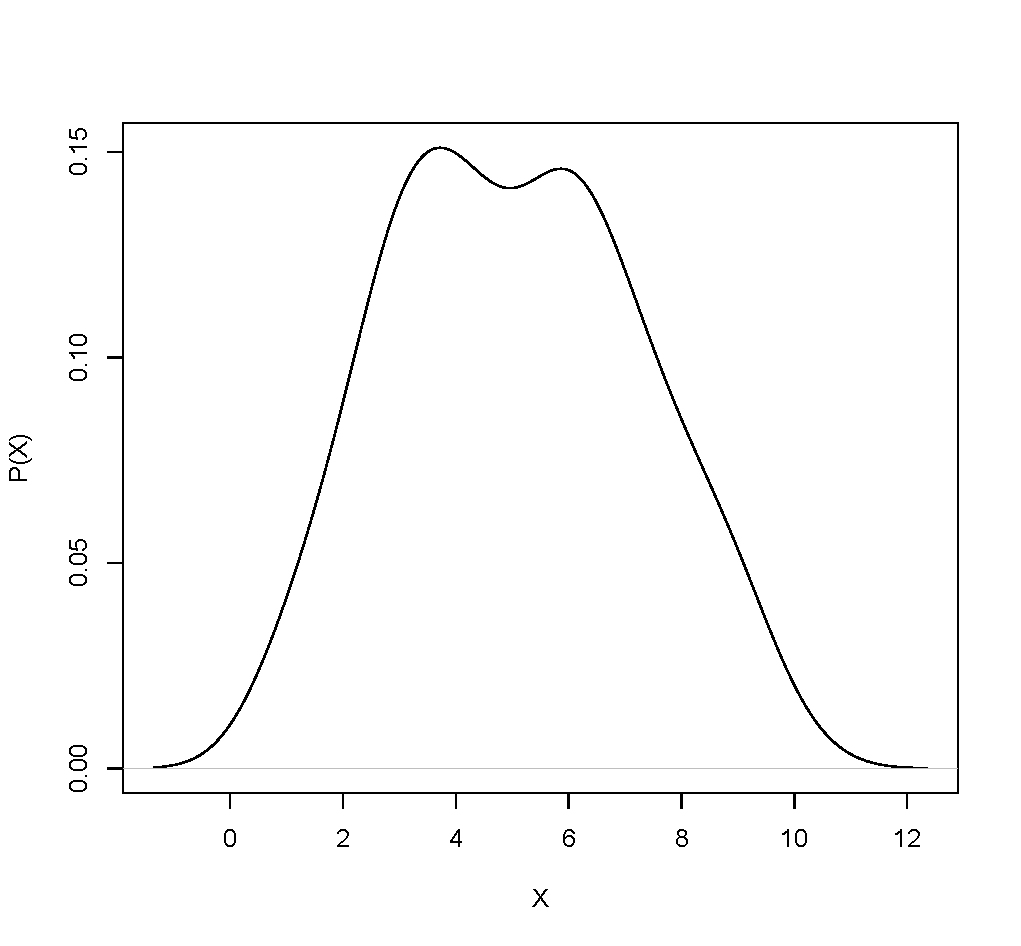
\includegraphics{DensityPlot.pdf}}
%\label{fig:nonfloat}
%\end{center}
\item How many dimensions does the probability distribution $P(y_1, ..., y_n | \beta)$ have? (A) 2 (B) n (C) n+1 (D) n+2  \index{Probability Review}
\item Why is the total jello in Gary's example equal to one?  \index{Probability Review}
\item In order to go from $P(y|\beta)$ to the $P(\beta|y)$, what do you have to add?  Does the $P(\beta|y)$ tell you about the probability of $\beta$ or the probability of $y$? \index{Maximum Likelihood}
\item What base of logarithm should be used to transform the likelihood function?  (A) 10 (B) e (C) 1  Bonus: Why? \index{Maximum Likelihood}
\item What is the correct theory of inference? \index{Theories of Inference}
\end{enumerate}

\subsubsection{Medium Questions}
\begin{enumerate}
\item Why is it computationally easier to take the log of the likelihood function? \index{Maximum Likelihood}
\item Fill in the blanks with the options below.  The log likelihood function is a \rule{10mm}{.1pt}, with one \rule{10mm}{.1pt} for each \rule{10mm}{.1pt}.  \\
sum, product, quotient, matrix, term, observation, factor, entry, book, variable (Taken from \emph{Statistical Models: Theory and Practice}) \index{Maximum Likelihood}
\item Identify the systematic and stochastic components for the Poisson model below.  \index{Maximum Likelihood}
\begin{eqnarray*}
Y_i &\sim& Poisson(\lambda_i) = \frac{\lambda_i^{y_i}\exp{(-\lambda_i)}}{y_i!}\\
\lambda_i &=& x_i\beta
\end{eqnarray*}
\item Why is one called systematic and the other stochastic? \index{Maximum Likelihood}
\item Explain why you have to go from $P(y|\beta)$ to the $P(\beta|y)$ in order to conduct inference. \index{Maximum Likelihood}
\item Is $P(y|\beta)$ the same distribution as $P(\beta|y)$?  Why or why not? \index{Probability Review}
\item Circle the terms in the log-likelihood below that you can drop before you solve for the MLE.\index{Maximum Likelihood}
\begin{eqnarray*}
\ln{L(\lambda|x)} = -\lambda n + \sum_{i=1}^n x_i\ln{\lambda} - \ln{(\prod_{i=1}^n x_i)}
\end{eqnarray*} 
\item What does it mean for an estimator to be \emph{unbiased}? \index{Properties of Estimators}
\end{enumerate}

\subsubsection{Hard Questions}
\begin{enumerate}
\item T/F Mary uses the same simple model we used in class, except she substitutes in an exponential distribution with parameter $\lambda$ for the stylized normal distribution with parameter $\beta$ that we had in class.  Her maximum likelihood estimate for $\lambda$ is still equivalent to the least-squares estimator. \index{Least Squares, Maximum Likelihood}
\item Mary tosses a coin three times and observes no heads.  She then gives the coin to John.  John tosses it until the first head occurs, and ends up tossing it 4 times total.  Let $\theta$ be the probability that the coin comes up heads.  What is the likelihood of $\theta$? ($3\theta(1-\theta)^6$) \index{Maximum Likelihood}
\item Suppose $X_i$ are independent for $i=1,...,n$ with common density $\frac{1}{2}\exp{(-|x-\theta|)}$, where $\theta$ is a parameter and $n$ is odd.   Without performing any calculations, what do you think the maximum likelihood estimate for $\theta$ will be and why? Hint:  It might be useful to think about the relationship between the model we solved in class and least-squares. (median) \index{Least Squares, Maximum Likelihood}
\item T/F The maximum likelihood estimate is always unbiased.  If you put true, explain why. If you put false, give an example of a case where the MLE is biased. \index{Least Squares, Maximum Likelihood} 
\end{enumerate}


\section{Lecture 3 -- Hour 2}
\subsection{A Simple Likelihood Model UPM Ch 4}
\subsubsection{Questions asked in Lecture}
\paragraph{20:38}  ``Would it be bias if you were trying to say you want to know if something is different from zero, would that be biased?" Follow-up:  ``If you were searching for significance that would be bad."
\paragraph{37:55}  ``So I can understand that all the distributions will get to the normal and that's why we can use this in a lot of cases, but why don't we do the log-likelihood for each respective distribution?"
\paragraph{39:10} ``Can one actually compare likelihoods from different models, say for example, this is generated by a normal distribution, or this is generated by a Poisson distribution."  ``So I couldn't test lets say comparing the log likelihood for a normal model and the log likelihood for a Poisson model."

\subsubsection{Easy Questions}
\begin{enumerate}
\item What ingredients (jello, food coloring, etc) would you need to make a likelihood function with four parameters, $y_1, y_2, y_3, y_4$?  Describe how you would use these ingredients to find the value of the likelihood at $y_1=1, y_2=2, y_3=3$ and $y_4=4$. \index{Maximum Likelihood, Probability}

\item How does the MLE help us summarize a likelihood of many dimensions?  \index{Properties of Maximum Likelihood Estimators}

\item Explain in 2-3 sentences what the curse of dimensionality is. \index{Probability}

\item What is the difference between solving for the MLE analytically and numerically? \index{Maximum Likelihood}

\item T/F If the second derivative of the likelihood at the MLE is negative, you know that the MLE is a maximum. \index{Maximum Likelihood, Math Review}

\item T/F If the second derivative of the likelihood at the MLE is negative, you know that the MLE is a global maximum. \index{Maximum Likelihood, Math Review}

\item Explain in 2-3 sentences what invariance to reparameterization allows you to do while calculating the MLE. \index{MLE - Invariance to Reparameterization}

\item T/F Invariance to sampling plans applies to both likelihood and to Neyman-Pearson hypothesis testing. \index{MLE - Invariance to Sampling}

\item Define the Law of Large Numbers and the Central Limit Theorem.  Do they contradict each other?  Why or why not? \index{Law of Large Numbers, Central Limit Theorem}

\item What are the three ways Gary discussed in class that can help you determine how well the MLE summarizes the likelihood? \index{Properties of Maximum Likelihood Estimators}

\item What is a nested restricted model?  \index{Likelihood Ratio Test}

\item What is the expected value of the Neyman-Pearson statistic when there is no difference between the restricted and unrestricted models?  \index{Likelihood Ratio Test}

\item Why is the likelihood ratio test powerful?  What is its disadvantage?  \index{Likelihood Ratio Test}

\item T/F As n gets larger the likelihood gets flatter. \index{Maximum Likelihood}

\item T/F As $\sigma^2$ gets larger the likelihood gets flatter. \index{Maximum Likelihood}
\end{enumerate}

\subsubsection{Medium Questions}
\begin{enumerate}
\item Circle the true statements.  A and B are random variables.  (A) $E(A + B) = E(A) + E(B)$  (B) $E(cA) = cE(A)$ where $c$ is constant  (C)  $E(A/B) = E(A)/E(B)$  (D) $E(A^2) = (E(A))^2$ Bonus: Under what condition is $E(AB) = E(A)E(B)$? \index{Probability}

\item Sometimes statisticians reparameterize the normal distribution, replacing $\sigma^2$ with $\xi$, where $\xi = 1/\sigma^2$ and is called the \emph{precision}.  The normal density then is
\begin{eqnarray*}
f(x|\theta, \xi) = \left(\frac{\xi}{2\pi}\right)^{1/2} \exp{\left(-\frac{1}{2}\xi(x-\theta)^2\right)}
\end{eqnarray*}
If the maximum likelihood estimate of $\sigma$ is $\hat{\sigma} = \sqrt{\frac{1}{n} \sum_{i=1}^{n} (X_i - \bar{X})^2}$, without maximizing the likelihood, what do you expect the MLE for $\xi$ will be? \index{MLE - Invariance to Reparameterization}

\item It can be shown under reasonable conditions that an MLE $\beta$ is a \emph{consistent} estimate of the underlying parameter $\mu$, that is, $\beta$ converges to $\mu$ in probability as $n$ approaches infinity.  What law/theorem/rule of MLE's we learned in class would be essential to this proof?  (A) Law of Large Numbers (B) Invariance to Sampling (C) Central Limit Theorem \index{Properties of Maximum Likelihood Estimators}

\item In lecture, $\sigma^2$ in the normal model summarizes (A) the curvature of the likelihood (B) the variability of the data (C) the variability of the MLE.  \index{Maximum Likelihood}

\item Using $\frac{-n}{2\sigma^2}$ as a summary of the likelihood when the data are not normal will be a better estimate when (A) $\sigma^2$ is smaller (B) n is larger (C) n is smaller. \index{MLE - Standard Errors}

\item When finding the MLE for $\sigma$ in a normal distribution, we have to make sure that the MLE for $\sigma > 0$ since the variance cannot be negative.  However, if you tell the computer to maximize $\sigma$, since the computer does not know the bounds on $\sigma$, it might output a negative number.  How could you reparameterize $\sigma$ so that the computer's output will translate into a positive MLE for $\sigma$? \index{MLE - Invariance to Reparameterization}

\item When is the likelihood ratio $\frac{L^*_R}{L^*}$ less than or equal to 1?  (A) When the restricted model is a better model.  (B) When the unrestricted model is a better model.  (C) Always -- the likelihood of the unrestricted model will always be greater than or equal to than the likelihood of the restricted model.  \index{Likelihood Ratio Test}

\item Mary wants to use the log-likelihood ratio test to determine whether she should use a restricted model where one of her parameters, $\beta_1=0$, or an unrestricted model where $\beta_1$ is estimated by the model.    For the restricted model, she calculates a log-likelihood value $L^*_R=-96.21$, and for the unrestricted model, she calculates a log-likelihood value $L^*=-84.71$.  Therefore, she calculates a likelihood ratio $\hat{R} = 2(-84.71 - -96.21) = 23$.   Using the Neyman-Pearson hypothesis testing framework, which model should she choose?  Hint: You will need to use the chi-square table and determine the test's degrees of freedom. \index{Likelihood Ratio Test, Hypothesis Testing}

\end{enumerate}

\subsubsection{Hard Questions}
\begin{enumerate}
\item Is the MLE asymptotically unbiased?  What law/theorem/rule would be important in proving this? \index{Properties of Maximum Likelihood Estimators}
\item Given what we learned in lecture today, what would you guess the asymptotic variance of the MLE is?  \index{MLE - Standard Errors}
\item T/F There can be more than one unbiased estimate of a mean $\mu$.  If so, give an example of two unbiased estimates of $\mu$.  If not, explain why not. (Yes, there can.  Sample mean of n data points, sample mean of n-1 data points.  But you're looking for the minimum-variance unbiased estimate, which is the MLE.)\index{Properties of Maximum Likelihood Estimators}
\item There are instances where you will want to find the maximum likelihood estimate for a parameter, $\theta$, where $\theta$ can only take on values between zero and one.  You will tell the computer to maximize this parameter, but unless you specify bounds the computer might return an impossible output, for instance an MLE that equals 2.  How could you reparametrize $\theta$ so that the computer's output will translate into a MLE between zero and one? \index{MLE - Invariance to Reparameterization}
\item Does the log-likelihood test tell you the probability that your restricted model is correct given the data?  Why or why not?  (What I'm trying to get at here is the discussion of hypothesis testing on pg 86 of UPM.  There might be a better question to get at this though.) \index{Likelihood Ratio Test, Hypothesis Testing}
\item Let $X_1, \ldots, X_n$ be a random sample from a Normal distribution with mean $\mu$ and variance $\sigma^2$.  The MLE for $\sigma^2$ is 
\begin{eqnarray*}
\frac{1}{n}\sum_{i=1}^n (X_i-\bar{X})^2
\end{eqnarray*}
If this is the maximum likelihood estimate, why do we often use $\frac{1}{n-1}\sum_{i=1}^n (X_i-\bar{X})^2$ instead? \index{Properties of Maximum Likelihood Estimators}
\item T/F If $X_n$ converges to a constant $c$ in probability and if $g$ is a continuous function, then $g(X_n)$ converges to $g(c)$ in probability.  In other words, if we know that $\bar{X}$ converges in probability to $\mu$ as $n$ gets large, does $\bar{X}^2$ converge to $\mu^2$ as $n$ gets large? \index{Law of Large Numbers}
\item T/F Say X is a random variable and is distributed $X \sim p(X|\theta)$.  Now let Y be another random variable where $Y = g(X)$.  $Y \sim p(g(X)|\theta)$.  \index{Probability}
\end{enumerate}

\section{Lecture 4 - Hour 1}
\subsection{Standard Errors and the Likelihood UPM Ch 4}
\subsubsection{Questions asked in Lecture}
\paragraph{10:01}  ``A hill."
\paragraph{10:19}  ``I just want to go back to where the log-likelihood is not normal you can still use a quadratic approximation because of the Central LImit Theorem? or because.."
\paragraph{11:55}  ``So it seems like we're sort of dancing around the Central Limit Theorem here in saying why the..so the likelihood is the density of not the log-likelihood but the likelihood is some constant we don't know and don't care about times the joint density of the data. And if we're talking about the joint density of say a sample mean or of the mean itself then we can be talking about the Central Limit Theorem in terms of why the distribution of our theta would be normal, but the distribution we're talking about is actually the distribution of the $y_i$'s not the mean of the $y_i$'s"
\paragraph{18:15} ``It's the variance from the second derivative".  ``If you take the square root of it that's the average amount that a random draw from that variable will deviate from the man."
\paragraph{19:25}  ``I'm a little confused -- I'm just trying to figure out.  I just I feel like I missed something so I'm a little lost at this point but are these standard deviations and standard errors among the data of our independent variables, right?"
\paragraph{21:32}  ``It's ahh variation in the variables of one explained by the others."
\paragraph{21:59}``How much one variable varies by the other variable if you were to draw multiple data samples and analyze what the standard deviation was across all of those samples."
\paragraph{23:19}  ``So you to be very succinct you would say common variability." ``So the square of the covariance is their common variability."
``I was just going to ask, so we have these datasets, you have all these different datasets, the diagonal ones are telling you...and for each of the datasets there will be a variance for each of the parameters.  The diagonal numbers are -- how do the diagonal numbers relate to the variances in each of the datasets?"
\paragraph{25:22} ``For instance in the stock market that measure represents like.. it's a very important measure for risk in the stock market"  ``Because if you are minimizing your risk you want one stock going in the opposite direction or like not moving together.  So in the market if one sector goes down, your portfolio is still going up."
\paragraph{30:43} ``This may be a silly question but is that variance-covariance matrix only a triangular matrix of the values?"

\subsubsection{Easy Questions}
\begin{enumerate}
\item How does the shape of the likelihood relate to the standard error of the MLE? \index{}

\item What term in a quadratic equation summarizes the curvature of the function? \index{MLE - Standard Errors}

\item T/F When you have a larger $\sigma$ for your data, you will need a bigger n to get the same standard errors as before. \index{MLE - Standard Errors}

\item Put circles around the variance terms of the variance-covariance matrix and put squares around the covariance terms of the variance-covariance matrix below. \index{Variance and Covariance}
\[\left(\begin{array}{ccc}
a & b & c \\
d & e & f \\
g & h & i \end{array} \right) \]
\item Explain what a standard error and a covariance are substantively. \index{Variance and Covariance}

\item T/F When the covariance between A and B is positive, when A is high in a dataset, B is low. \index{Variance and Covariance}

\item I am estimating two parameters, $\mu$ and $\sigma$ with MLE's $\hat{\mu}$ and $\hat{\sigma}$.  Draw a variance covariance matrix and indicate what each of the entries in the matrix would represent. \index{MLE - Standard Errors, Variance and Covariance}
\end{enumerate}

\subsubsection{Medium Questions}
\begin{enumerate}
\item T/F As n gets larger, data distributed Exponential will be become Normally distributed. \index{Central Limit Theorem}

\item T/F As n gets larger, the mean of data distributed Exponential will become Normally distributed. \index{Central Limit Theorem}

\item T/F The curvature of the likelihood is a summary of the variability of the MLE across datasets. \index{MLE - Standard Errors}

\item To estimate the variance of the difference between two parameters, say $\hat{\beta}_1 - \hat{\beta}_2$ you will need (circle all that apply) (A) the point estimates (B) the variance of $\beta_1$ (C) the variance of $\beta_2$ (D) the covariance of $\beta_1$ and $\beta_2$. \index{Variance and Covariance}

\item The Wald Test is a test to explore the precision of the MLE.  The Wald Test can be calculated as: $W = \frac{\hat{\beta} - \tilde{\beta}}{\hat{\sigma}}$, where $\hat{\beta}$ is the maximum likelihood estimate, $\tilde{\beta}$ is the hypothesized value of $\beta$ and $\hat{\sigma}$ is the standard error of $\hat{\beta}$.  Without performing any calculations, how do you think this test statistic is distributed?  Alternatively, the Wald Test can be calculated $W^2$.  How do you think this test statistic would be distributed?  Why? \index{Wald Test, Hypothesis Testing}
\end{enumerate}

\subsubsection{Hard Questions}
\begin{enumerate}
\item The likelihood ratio test is considered \emph{most powerful} (power greater than all other tests for a given significance level $\alpha$)  when testing a simple hypothesis vs. a simple hypothesis.  However, for cases when there are many hypotheses, or under a composite alternative, this property no longer holds.  Why do you think this is?  What statistics other than the likelihood ratio test would you use to describe how well your MLE describes the data if you wanted to test composite alternatives? \index{Likelihood Ratio Test, Hypothesis Testing}
 
 \item What is the difference between a consistent estimator and an unbiased estimator?  Which property do you find more desirable in an estimator? \index{Properties of Maximum Likelihood Estimators}
 
 \item The mean squared error of an estimator is defined as:
 \begin{eqnarray*}
 MSE(\hat{\mu}) = Var(\hat{\mu}) + \left(Bias(\hat{\mu}, \mu)\right)^2 
 \end{eqnarray*}
 How does this equation show a bias-variance trade-off?  What do you think is more important in an estimator -- low bias, or low variance? \index{Properties of Maximum Likelihood Estimators}
 
 \item Compare the maximum likelihood theory of inference and least squares.  Which approach is more general?  Why?  Which approach do you find more philosophically justifiable?  Why? \index{Least Squares, Maximum Likelihood}
 
 \item Describe the four steps you would use to analytically solve for the maximum likelihood estimate. \index{Maximum Likelihood}
 
 \item If you had to develop a computer program to numerically find the maximum likelihood estimate, how would you design it?  You have two goals in mind: accuracy and computational efficiency. You are given the likelihood function and a vector of starting values for the parameters. \index{Maximum Likelihood}
  
 \item By the Central Limit Theorem, as n approaches infinity, any maximum likelihood estimate $\beta$ is distributed approximately normal with mean $\mu$ and variance $1/[nI(\mu)]$, where $I(\mu)$ is called the Fisher Information.  Using what we learned in class today, what do you expect the Fisher Information of $\mu$ in the the normal distribution to be? \index{MLE - Standard Errors}
 
 \item Follow-up from above question.  What does it mean for a matrix to be positive-definite?  Why would it be important that the Fisher Information matrix be positive definite? \index{MLE - Standard Errors, Math Review}
 
 \item Two estimates of $\eta$, $\hat{\eta}$ and $\tilde{\eta}$ are unbiased. Thus the \emph{efficiency} of $\hat{\eta}$ relative to $\tilde{\eta}$ equals\footnote[1]{ When estimates are unbiased, the mean squared error of the estimate equals the variance of the estimate, therefore the efficiency can be expressed in terms of the variance.}
\begin{eqnarray*}
eff(\hat{\eta}, \tilde{\eta}) = \frac{Var(\tilde{\eta})}{Var(\hat{\eta})}
\end{eqnarray*}
Knowing what you do about the desirable properties of estimators, which estimator would you choose to use if $eff < 1$?  What about if $eff >1$? Why?
\item The Cramer-Rao Inequality states that when $X_1,\ldots,X_n$ is i.i.d. with density function $f(x|\theta)$, and $T=t(X_1,\ldots,X_n)$ is an unbiased estimate of $ \theta$, then Var(T) $\geq \frac{1}{nI(\theta)}.$ An \emph{efficient} estimate is an unbiased estimate whose variance achieves this lower bound $\frac{1}{nI(\theta)}$.  These two rules combined prove that the MLE is always (A) efficient (B) asymptotically efficient.  \index{MLE - Standard Errors}
 
 \item What does it mean for an estimator to be minimum variance unbiased?  Why is this a desirable property? \index{Properties of Maximum Likelihood Estimators}
 
 \item T/F The unbiased minimum variance estimator is the estimator with the smallest mean squared error. \index{Properties of Maximum Likelihood Estimators}  
\end{enumerate}

\subsection{Simulation of the Maximum Likelihood Model}
\subsubsection{Questions asked in Lecture}
\paragraph{36:32}  ``Is theta normal because theta is .. I'm confused about whether theta is a data piece or a statistic of the data and that's why it becomes normal."  ``That's just the Central Limit Theorem."
\paragraph{37:32}``If we knew the distribution of the $y_i$'s, like the numbers in the datasets, then should we be using the multivariate binomial distribution instead of the multivariate normal? I mean because we're now talking about the estimator, not the data." ``If you didn't want to do that.."
\paragraph{39:12} ``So one of the earlier slides on the properties of the MLE you talk about how as n goes to infinity the MLE is collapsing over b,  which spikes, so it was the MLE over the standard error that is normal. That isn't what this is because that's what I was thinking of."

\subsubsection{Easy Questions}
\begin{enumerate}
\item To simulate parameters from a multivariate normal, what assumption do we have to make? \index{Simulation}
\item T/F We have to assume that the stochastic component of our model is normal in order to use simulation to estimate the parameters. \index{Maximum Likelihood, Simulation}
\item If you take one draw from a three dimensional multivariate normal, how big will the vector output be? \index{Simulation}
\end{enumerate}

\subsubsection{Medium Questions}
\begin{enumerate}
\item If $Y_i \sim f(y|\mu, \sigma^2)$ and $\epsilon_i = Y_i - \mu$, how is $\epsilon_i$ distributed?  What property of a Normally distributed variable do you need to prove this?  \index{Probability}
\item Rewrite the likelihood of a normal replacing all $Y_i$'s and $\mu$'s with $\epsilon_i = Y_i - \mu$. \index{Maximum Likelihood}
\end{enumerate}

\subsection{Forcasting Presidential Elections}
\subsubsection{Questions asked in Lecture}
\paragraph{46:49}  ``Well if one state -- I take that back -- I was going to say if one state is a home state, then another state has a lower probability of being a home state but that's a covariate."
\paragraph{47:01} So we're saying that the mean of a state at any given time is independent, so let's say California, that fact that California voted for a Democrat in one election is completely independent in any other year."  ``Yeah, in California".
\paragraph{47:36} ``It doesn't look like in the notes that we're going to get to this today, but what do we do to calculate heteroskedastic consistent standard errors in the likelihood model,  I know that the white stuff is all for OLS, right?"  "It clearly presupposes something we're trying to avoid presupposing." 
\paragraph{49:15} ``Yes."
\paragraph{54:23} ``So I just want to be really clear when you have the plus two and k + 2 is that the intercept and sigma?"
\paragraph{56:50} ``What about the intercept?"

\subsubsection{Easy Questions}
\begin{enumerate}
\item What is an ancillary parameter? \index{Maximum Likelihood}
\item In the election example, what do we want to calculate?  How is that different from the statistics that come out of the model?  \index{Quantities of Interest}
\item Mary decides to change the election forecasting model from $Y_{it} \sim N(\mu_{it}, \sigma^2)$ to $Y_{it} \sim N(\mu_{it}, \sigma_{it}^2)$.  How has she substantively changed the model? \index{Maximum Likelihood}
\item Identify two problems with the election model from class. \index{Election Example}
\item Why are there two products in the likelihood function of the election example? \index{Maximum Likelihood, Election Example}  
\end{enumerate}

\subsubsection{Medium Questions}
\begin{enumerate}
\item Why do we substitute in $X_{it}\beta$ for $\mu_{it}$ in the log-likelihood function?  Why couldn't we just leave it with $\mu_{it}$?  \index{Maximum Likelihood}
\item T/F $\prod_{i=1}^n\prod_{t=1}^T L(y_{it}|\mu_{it}, \sigma^2) = \prod_{t=1}^T\prod_{i=1}^nL(y_{it}|\mu_{it}, \sigma^2)$ \index{Math Review}
\item What are the parameters in the election model?  How many are there? \index{Election Example}
\end{enumerate}

\section{Lecture 4 - Hour 2}

\subsection{Forcasting Presidential Elections -- Ch 4 UPM}

\subsubsection{Questions asked in Lecture}
\paragraph{7:22} ``People do it, I mean, if there are critical prediction rules, I mean, that's how they make them."
\paragraph{7:29} ``I'm not sure if this is right, but wouldn't that sort of affect.. that you're essentially using data from each state ... each state is a different trial... and in that circumstance there's no .. ummm.. like you might end up with them winning Nebraska under a simulation condition when it's rainy in Nebraska and that adding that to the number of electoral votes for Iowa when the weather in that simulation for Nebraska was sunny or something like that...am I off?"
\paragraph{8:18} ``You lose the uncertainty in that way, right, because beta hat is predicted and has some uncertainty."  
\paragraph{8:46} ``Yeah.. I think that in one state your point estimate is that you are going to get .51 or something like that and you have a very small confidence interval around it then it might be kind of...like a really really tiny confidence interval... then you might be certain that even though it's .51 it's going to be ok but had you known that there was a large confidence interval around it, then you might not be sure about how that's state's going to turn out which might mess up your predictions."
\paragraph{17:10} ``How many electoral college votes did Clinton get?" 
\paragraph{17:37} ``370" ``He got 43\% of the popular vote.."
\paragraph{18:04} ``53 \%."
\paragraph{18:10} ``This is the electoral vote.  He got 69 \% of the electoral vote."
\paragraph{18:55} ``When you reparameterize sigma, presumably the reason you get away with that is that the crest of the hills on that function have a one-to-one correspondance to the hills on sigma, right, that's why you can get away with that." ``Ok, so, but presumably that..er..that's going to affect how the optimization procedure works, it's going to essentially going to change where the answer is, right, you get the same answer in the end."
\paragraph{26:05} ``I was just going to ask..so if..for both three..so is there uncertainty in the estimate of $\sigma_{it}^2$?" ``But sorry in other words.. the only.. there is no residual term on.. in the estimate of the variance i,t there is no..it's completely predicted by the covariates that we have on z." ``Shouldn't we have a stochastic and a stochastic?"
\paragraph{28:44} ``Is gamma which gets at the variance an ancillary parameter in this model, or is it because it's tied to i and t now."

\subsubsection{Easy Questions}
\begin{enumerate}
\item What types of summary statistics might we be interested in from the electoral model? \index{Election Example}
\item Explain in 2-3 sentences what a predictive distribution is. \index{Prediction}
\item Why do we want the distributions of the quantities of interest rather than just the quantities of interest?  \index{Quantities of Interest}
\item Explain what is wrong with using the point estimates from the model to predict who wins the election. \index{Prediction}
\item Why do we get different predictions from each simulation?  What two types of uncertainty create differences in predictions?  Explain the difference between them. \index{Prediction, Simulation}
%\item Based on this posterior distribution, what would you say is the percent chance that the Democrats will win the election? \index%{Prediction}
%\begin{center}
%\scalebox{0.4}{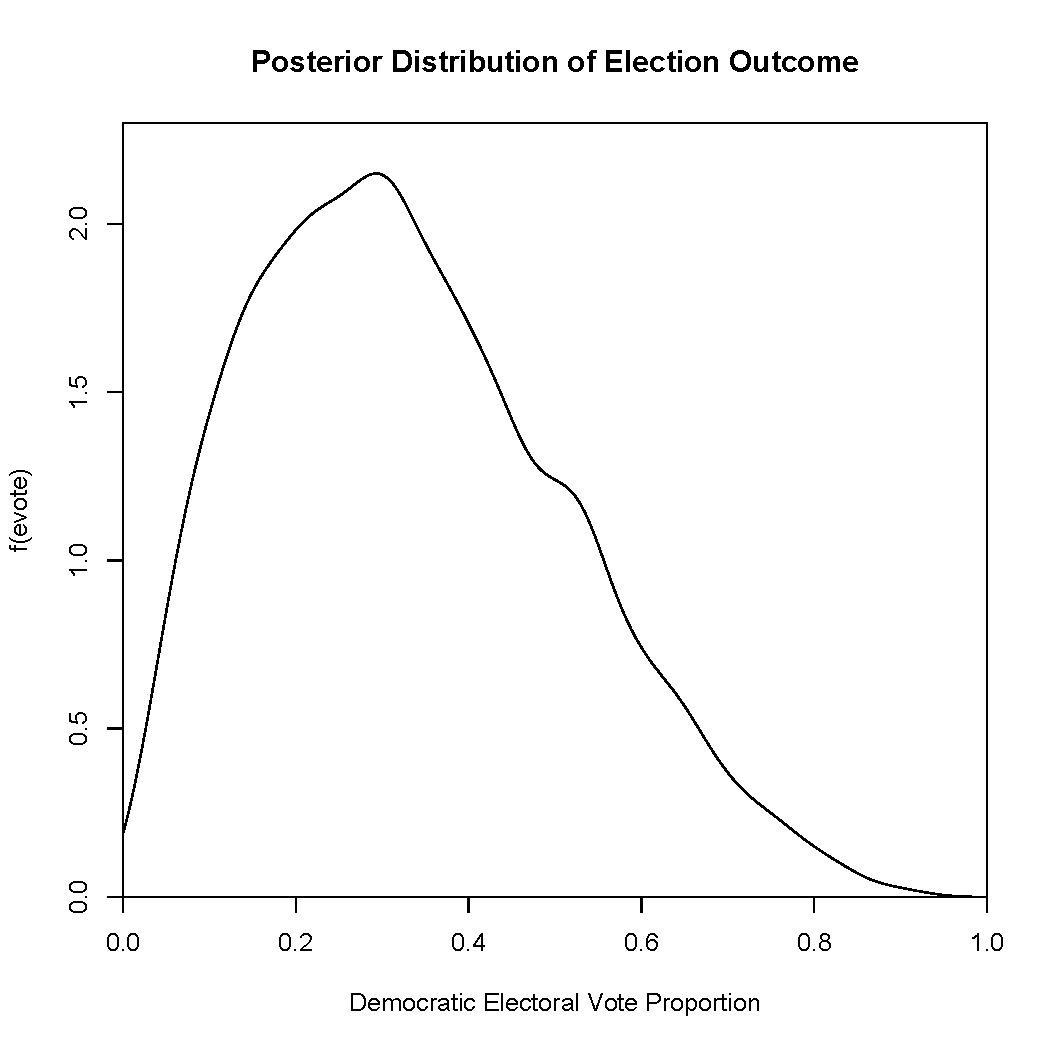
\includegraphics{ElectionPosterior.pdf}}
%\label{fig:nonfloat}
%\end{center}
\item Write out the steps in drawing simulations of $y_{i, 2008}$.  \index{Simulation, Election Example}
\end{enumerate}

\subsubsection{Medium Questions}
\begin{enumerate}
\item Mary wrote a model similar to the election model in class, but she parameterized $\sigma_{it} = \exp{(\alpha_0 + \alpha_1S_i)}$, where $S_i$ is the number of people surveyed each year in the polls that are included in the covariate matrix.  What sign would you expect the maximum likelihood estimate of $\alpha_1$ to have?  Why? \index{Maximum Likelihood, Election Example}
\item List two or three variables you would include in $z_{it}$ of the systematic component, $\sigma_{it} = \exp{(z_{it}\gamma)}$, in the electoral model. \index{Maximum Likelihood, Election Example}
\item A probit model for reading says that subject $i$ read a book last year if $X_i\beta + U_i > 0$.  Circle all that apply $U_i$ is a \rule{10mm}{.1pt} variable.  (A) data (B) random (C) latent (D) dummy (E) observable.  \index{Prediction}
\item (Follow-up from previous question.)  Using the model, could you predict with certainty that someone from the sample will read a book next year? \index{Prediction}
\item Suppose you did what Gary said not to do -- ran regressions on each state and predicted a win for the Democrats in every state where the predicted probability was above 0.5.  Under what conditions would this be most problematic?  \index{Prediction}
\end{enumerate}

\subsubsection{Hard Questions}
\begin{enumerate}
\item How could you take a parameter that varied from $(0, \infty)$ and reparametrize it so it could be interpreted as partisan bias?  (pg 76 of UPM). \index{MLE - Invariance to Reparameterization, Election Example}
\item Say you had data on the outcomes of two exit polls from $n$ elections.  You assume in your model that each election the outcome has a different mean, but the variance between elections is the same.  Therefore, your model specification is:
\begin{eqnarray*}
Y_{ji} \sim N(y_{ji}|\mu_i, \sigma^2)
\end{eqnarray*}
where $j=1,2$ and $i=1,...n$.  You want to estimate $\sigma^2$, in other words $\mu_i$ is an ancillary parameter.  Why will you run into problems estimating the MLE for $\sigma^2$?  Will your estimates for $\sigma^2$ be consistent?  Bonus:  How could you solve this problem? (Taken from UPM.) \index{MLE Pitfalls}
\item Suppose there are $N$ balls labeled 1,2,\ldots,$N$ with unknown distinct values $\theta_1,\ldots,\theta_N$ written on them.  Draw $n$ balls at random without replacement (where $n < N$) and observe ($a_i,b_i$) for $i=1,2,\ldots,n$, where $a_i$ is the number of the $i$th ball drawn and $b_i$ is the value $\theta_{a_i}$ written on the ball labeled $a_i$.  Now consider estimating the parameter $\theta = \theta_1 + \cdots+ \theta_N$.  What is the likelihood of $\theta_1, \ldots, \theta_N$?   Why is the likelihood problematic?  (Adapted from \emph{Counterexamples in Probability and Statistics}.  Likelihood of $\theta_1,\ldots,\theta_N$ will be ${N \choose n}^{-1}$.  Same problem as above exists -- because there are more parameters than data values, the likelihood is uninformative.)  \index{MLE Pitfalls}
\item Charlie has already estimated his maximum likelihood estimates for his election polling data, but just got some more money so is planning on collecting some new polling data and combine it with his old data.  However, Mary tells Charlie he can't do this, giving an example to prove her point. Mary says, say I had one set of data (12,13,14) and another set of data (20,21,22) that come from a Normal distribution with mean $\mu$ and variance $\sigma^2$.  The MLE for $\sigma^2$ from the first set of data is $2/3$ and the MLE for $\sigma^2$ from the second set of data separately is $2/3$. However, when you combine them the MLE for $\sigma^2$ is $50/3$.  Therefore, she says, $\sigma^2$ is obviously not invariant to resampling.   Explain why Mary is wrong and justify why the property invariance to resampling still holds.  \index{MLE - Invariance to Sampling}
\item Just as we can use simulation to predict the probability of the Democrats winning an election, we can use Monte Carlo simulation to solve hard math problems, for example taking difficult integrals.  Suppose for a second that you can not analytically solve the integral $I = \int_{0}^{1}x^3dx$.  How could you solve this numerically using simulation? (Simulate numbers on Unif(0,1), evaluate them at $x^3$, take the average.) \index{Simulation}
\item (Similar to above).  The integral of the standard normal density from 0 to 1, $I(f) = \frac{1}{\sqrt{2\pi}} \int_{0}^{1} \exp{(-x^2/2)}dx$ cannot be evaluated in closed form.  Use the sampling technique you described above to evaluate the integral. \index{Simulation}
\item Let $Y_{it}$ be the number of accidents a driver $i$ is involved in on day $t$ and $X_{it}$ be the speed of driver $i$ on day $t$.  You want to study the relationship between $Y_{it}$ and $X_{it}$.  To do this, you consider using a least squares model where:
\begin{eqnarray*}
Y_{it} = \beta_0 + \beta_1X_{it} + \epsilon_{it}
\end{eqnarray*}
A statistician notes that your data $Y_{it}$ are probably distributed Poisson because an accident is a rare event.  The statistician suggests that before running your regression, you transform $Y_{it}$ into $\sqrt{Y_{it}}$ because the square root of a Poisson random variable has a variance that is independent of the mean and approximately constant.  Why would this be important for a Poisson dependent variable?  Can you think of a better solution than the statistician proposed? \index{Maximum Likelihood Models}
\item Under certain conditions, the Binomial distribution with probability of success $p$ can be approximated by a normal distribution.  For what values of $p$ do you think this approximation would be best? How would the approximation be affected by $n$?  Hint: A rule of thumb is that the approximation is reasonable when $np > 5$ and $n(1-p)>5$.  \index{Probability}
\end{enumerate}

\subsection{Binary Variable Regression Models -- pg. 97-110 UPM} 
\subsubsection{Questions asked in Lecture}
\paragraph{36:15} ``Optimize it."
\paragraph{36:52} ``Plug them back into the formula for $\pi$."

\subsubsection{Easy Questions}
\begin{enumerate}
\item Give two examples of political data that could be modeled with a Bernoulli distribution. \index{Binary models}

\item Identify the stochastic and systematic components of the logistic regression model.  \index{Logit models}

\item List two problems with using a linear regression model in place of a logistic regression model. \index{Logit models}

\item Would you include the $\beta$'s from a logistic regression in your regression table? Why or why not? \index{Logit models}

\item Describe two good ways of presenting results from a logistic regression. \index{Logit models, Interpreting data}

\end{enumerate}

\subsubsection{Medium Questions}
\begin{enumerate}
\item The graph below plots logit curves where:
\begin{eqnarray*}
\pi_i = \frac{1}{1 + \exp{(\beta_0 + \beta_1x_i)}}
\end{eqnarray*}
Match the coefficients for $\beta$ with the curve. (A) $\beta_0=0, \beta_1=1$ (B) $\beta_0=0, \beta_1=0$ (C) $\beta_0= 1, \beta_1=-3$ (D) $\beta_0 = 2, \beta_1=1$.  How does the $\beta_0$ affect the curve?  How does $\beta_1$ affect the curve? \index{Logit models}

%\begin{center}
%\scalebox{0.4}{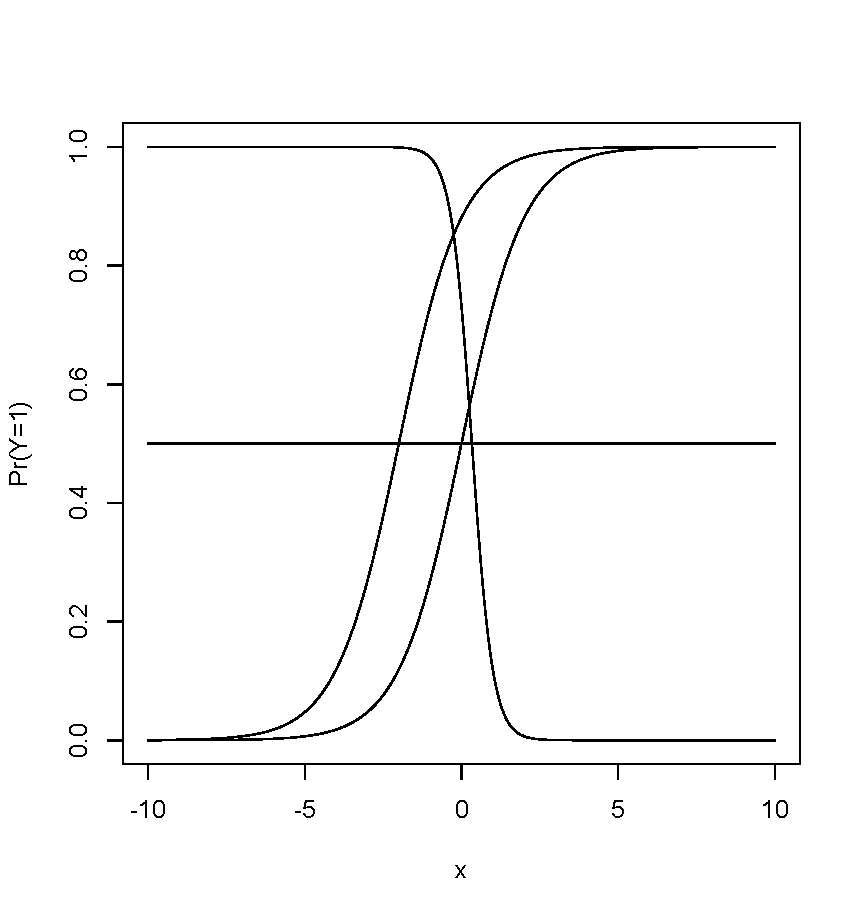
\includegraphics{LogisticPlot.pdf}}
%\label{fig:nonfloat}
%\end{center}

\item The logistic curve was originally used to model population growth (Verhulst 1845, Yule 1925).  List two reasons why using this model would make sense in the context of population growth.  In 1920, the population of the United States was 106 million and models based on the logistic curve showed that the population would never exceed 200 million.  Despite your reasons why using the logistic curve would make sense, why do you think it failed in the end?  (Info taken from \emph{Statistical Models in Theory and Practice}). \index{Logit models}

\item Take the derivative of 
\begin{eqnarray*}
\hat{\pi} = \frac{1}{1 + \exp{(\hat{\beta_0} + \hat{\beta_1}x_1 + \hat{\beta_2}x_2)}}
\end{eqnarray*}
with respect to $x_2$.  Substitute $\hat{\pi}$ back in the derivative so your derivative is in terms of $\hat{\beta_2}$ and $\hat{\pi}$. How does the derivative vary over $\hat{\beta_2}$ and over $\hat{\pi}$?  How does this equation help you substantively interpret $\hat{\beta_2}$? \index{Interpreting data}

\item An alternative representation of a binary regression model is where $Y_i^*$ is a continuous unobserved variable distributed $Y_i^* \sim f(y_i^*|\mu_i)$ with systematic component $\mu_i = x_i\beta$.  The observed $y_i$ is related to $Y_i^*$ by:
\begin{eqnarray*}
y_i = \Big\{ \begin{array}{cccc} 1 , y_i^* \leq \tau \\ 0 , y_i^* \geq \tau \\ \end{array}  
\end{eqnarray*}
Give an example where this formulation makes sense.  Give an example where the original formulation makes more sense. \index{Binary models, Interpreting data}
\end{enumerate}


\section{Lecture 5 -- Hour 1}

\subsection{Binary Variable Models (continued from Lecture 4) (UPM pages 98-101 and 110-115)}

\subsubsection{Questions asked in Lecture}

\paragraph{04:40} ``How useful is this for...It seems like that the point of using this is that you have some archetypal types of people, male in Chicago, such that your population is near those archetypes. That information doesn't actually tell you how weird they are in terms of their outcome. It could be the case that male age 21 Chicago income 30000  probability of vote...."

\paragraph{27:25} ``The first step when we are assuming that things are normally distributed...it seems against the grain of what we've been doing so far. It seems like we try to find the functional form that best fits, but here we are assuming normality to make it work? (Follow up question: How do you know $Y^*$ is normally distributed?)"

\paragraph{31:31} ``You were saying that the original derivation is, well, maybe not assumption free, but, with, uh, more easily accepted assumptions. But isn't the difference that we're talking here not about stochastic components, but rather about the systematic component?  In that if we were to draw the difference between the logit and the probit it's about the linear assumption of the $\beta$'s...Is that true? Because otherwise if our derivation of the logit model was assumption free then we should be saying that probit is wrong?"

\paragraph{35:43} ``So if $Y^*$ is not observed then how does it make sense to calculate the probability of a specific $Y^*$, like, what does that mean, if you don't know what it is, then how can you...?"

\paragraph{36:12} ``Ok, so let's say with the bug example, that you know whether the bug is dead or alive, you don't know how healthy it is or how unhealthy is so later on when you do the derivation...and there are only two outcomes, why does it make sense to say what is the probability of any specific $Y^*$?"

\paragraph{49:30} ``I see a lot of papers that report the [unintelligible]. What is that?"

\paragraph{54:20} ``Is that you should be able to do it in one table or maybe if you took two tables? Because it could be that you put, like, the [unintelligible] the and then all of these variables in another table. So you should just be able to tell the story with all of the tables or just one table"

\subsubsection{Easy Questions}

\begin{enumerate}
\item Given an example of the kind of data that would be appropriately analyzed using a logit or a probit specification and explain why.  Two or three sentences is sufficient. \index{Binary variable models}
\item True/False.  Both the probit and the logit specifications have Bernoulli stochastic components. \index{Binary variable models}
\item True/False. In a binary variable model, $E(Y_i)=\hat{\pi_i}$. \index{Binary variable models}
\item Which of the following kinds of data are appropriately analyzed using a logit or a probit specification? (A) Heights of adult men measured in centimeters, (B) The number of executive orders the President signs into law per year, (C) Whether a person votes in a Presidential election, (D) The number of patents approved by the U.S. patent office per year, (E) None of the above. \index{Binary variable models}
\index{Binary variable models}
\item True/False.  The logistic systematic component, $\pi = \frac{1}{1+e^{-X_i\beta}}$, serves to constrain $\pi$ between 0 and 1. \index{Binary variable models}
\item Explain in 2-3 sentences the information provided by a first difference analysis.  Why is it useful? \index{Interpreting data ! First differences}
\item True/False.  In a binary variable model (such as a logit or a probit), we assume that $\pi$ (A) Varies over observations, (B) Does not vary over observations, (C) May or may not vary across observations. \index{Interpreting data ! First differences}
\item In lecture, Gary says that there are ``four ways of interpreting functional forms."  What are these four ways? \index{Interpreting data}
\item True/False. You can use a logit regression and a probit regression interchangeably because they will give you the \underline{exact same coefficient values}. \index{Binary models}
\item True/False. You can use a logit regression and a probit regression interchangeably because the \underline{inferences that you draw from them will be the same}, even though the exact coefficient values will differ. \index{Binary variable models}
\item True/False.  Under the alternate justification for binary variable models, the estimated $\tau$ value is substantively meaningless.\index{Binary models ! Logit models}
\item The best way to interpret a logit coefficient quickly is to (A) Interpret as you would a linear regression coefficient, (B) Interpret the coefficient value as indicating a percentage change in $Y$, (C) Multiply it by four, (D) Divide it by four, (E) None of the above. \index{Binary models ! Logit models}
\item When you multiply a probit coefficient by four, you get an estimate of (A) The variable's average effect,(B) The variable's minimum effect, (C) The variable's maximum effect, (D) Nothing; it's a non-sensical transformation. \index{Binary variable models ! Probit models}
\item When you multiply a logit coefficient by four, you get an estimate of (A) The variable's average effect,(B) The variable's minimum effect, (C) The variable's maximum effect, (D) Nothing; it's a non-sensical transformation. \index{Binary variable models ! Logit models}
\item You are a researcher studying patient fatality and smoking. You run a logit model with death in any given year (1 if death occurs, 0 if the patient is alive at the end of the year) as the dependent variable and smoking (1 if smoker, 0 if non smoker) as the only dependent variable. The computer program returns a coefficient of 1.2 on the smoking variable.  How do you interpret this? (A) The probability of death increases by 1.2 if you are a smoker, (B) The probability of death increases on average by 4.8 if a patient is a smoker, (C) At its maximum, probability of death increases by 4.8 if you are a smoker, (B) At its minimum the probability of death increases by 4.8 if you are a smoker, (C) None of the above.
\item In lecture, Gary identifies three justifications for the same binary variable model. What are they? \index{Binary variable model}
\item A researcher has fit a probit model to analyze the relationship between voter turnout (a yes or no variable) and gender, age, and race (black = 1, non-black = 0).  She wants to know the probability that a black 35-year old man will vote versus the probability that a white 35-year old man will vote.  Which of the ways of interpreting functional forms do you recommend to her? (A) First Difference analysis, (B) Interpreting the coefficient on the race variable using the derivative, (C) Graphing, (D) Calculating fitted values, (E) Some combination.
\item True/False. As in OLS, we can include interaction terms when working with logit and probit regressions.\index{Binary variable models}
\item True/False.  The logit and probit CDFs are exactly the same.\index{Binary variable models}
\end{enumerate}

\subsubsection{Medium Questions}

\begin{enumerate}
\item A researcher wants to analyze dichotomous data. She asks you whether she should use a logit regression or a probit regression to analyze the data. What should you tell her? (A) Logit, (B) Probit, (C) Neither, (D) Either, (E) It depends. \index{Binary Data}
\item True/False.  The inferences you can draw from the regular conceptualization of a logit model and the ``bug'' conceptualization of a logit model are the same. \index{Binary models ! Logit models}
\item True/False.  Although $X_i\beta$ is linear in $X$, the resulting probabilities from the logit model are not.\index{Binary models ! Logit models}
\item True/False.  Deriving a probit maximum likelihood estimate can be done analytically.
\item True/False. In a probit or logit model, a single unit change in $X_i$ will have a different effect on $\hat{\pi}$ depending on the points at which the curve is evaluated. \index{Binary variable models}
\item True/False. With a logit or probit stochastic component, the regression line is nonlinear. \index{binary variable models}
\item True/False. For values of $X$ that are close to their mean, using a linear model is probably okay because it is unlikely to yield values greater than 1 or less than 0. \index{Binary variable models}
\item As $\pi_i$ approaches one, then the rate at which it increases must (A) Slow, (B) Accelerate, (C) Stay the same, (D) It depends on the values of $X$. \index{Binary variable models}
\item Your friend is interested in looking at voter turnout (voted = 1, not voted = 0) and its potential relationship to ethnicity.  She mentions to you that everyone in her sample has voted -- so, everyone in her sample has a ''1'' for the dependent variable. Can your friend can extract inferences using a binary variable model of this data? (A) Yes, (B) No, (C) It depends \index{Binary variable models}
\item Your friend is interested in looking at voter turnout (voted = 1, not voted = 0) and its potential relationship to ethnicity (black = 1, non-black = 0).  She mentions to you that everyone in her sample is black -- so, everyone in her sample has a ``1'' for the explanatory variable. Can your friend can extract inferences using a binary variable model of this data? (A) Yes, (B) No (C) It depends \index{Binary variable models}
\item You are a researcher studying the heights of American men. You know that male height follows a normal distribution, but your data source only reports to you whether the subjects are taller or shorter than six feet tall, a dichotomous variable (six feet or greater = 1, under six feet = 0). What sort of model should you use to analyze these data? (A) Probit model, (B) Logit model, (C) Either probit or logit, (D) Linear regression model \index{Binary variable models}
\item True/False. There is a substantive difference between a normal distribution and a general standardized logistic distribution. \index{Binary variable models ! Logit models}
\item True/False. Even if you could observe $Y^*$, the latent unobserved variable, you would still want to analyze the effects of covariates using a binary variable model.
\end{enumerate}

\subsubsection{Hard Questions}

\begin{enumerate}
\item True/False. $E(Y_i)=\pi_i$ is never observed. % true -- UPM p 99, Y always 0 or 1 \index{Binary variable models}
\item In a probit or logit model, the effect of $X_i$ on $\hat{\pi_i}$ is greatest when $\hat{\pi}$ equals (A), 0, (B) 1, (C) 0.5, (D) It depends. \index{Binary variable models}
\item Your friend is interested in looking at the relationship between voter turnout (where voting = 1, and not voting = 0) and being black (where black = 1, not black = 0). She has no other variables in her model.  True/False: The inferences she obtains from running a linear regression analysis on these data will be exactly the same as the inferences she obtains from running a logit analysis.\index{Binary variable models ! Logit models}
\item Your friend works at major Boston research hospital. The hospital is doing an audit on patient mortality, and your friend has run a logit regression with whether a patient has died in the hospital in the calendar year (1 = patient has died, 0 = patient is alive) as the dependent variable and \underline{no independent variables}. The computer program returns a coefficient of .4 on the intercept variable and nothing else.  How should your friend interpret this coefficient? (A) the probability of dying in the hospital is .4, (B) 
\item The interpretation of a probit coefficient, $\beta_1$, is that a one-unit increase in the variable $X_1$ is linked with an (A) Increase in $Y^*$ by $\beta_1$ units, (B) Increase in $Y^*$ by $\beta_1$ percent, (C) Increase in $Y^*$ by $\beta_1$ standard deviations, (D) None of the above. \index{Binary variable models ! Probit models}
\item True/False.  Logit and probit regressions, just like linear regression, assume homoscedasticity. \index{Binary variable models}
\end{enumerate}

\subsection{Presenting Results (King, Tomz, Wittenberg) (last 5 minutes)}

\subsubsection{Questions Asked in Lecture}

\paragraph{49:30} ``I see a lot of papers that report the [unintelligible]. What is that?"

\paragraph{54:20} ``Is that you should be able to do it in one table or maybe if you took two tables? Because it could be that you put, like, the [unintelligible] the and then all of these variables in another table. So you should just be able to tell the story with all of the tables or just one table"


\section{Lecture 5 -- Hour 2}

\subsection{Presenting Results (continued) (King, Tomz, Wittenberg paper)}

\subsubsection{Questions asked in Lecture}

\paragraph{18:10} ``Could you say what $\theta$ is?"

\paragraph{18:57} ``With $\beta$'s and $\alpha$'s, yeah, why did you draw it from the normal distribution? 

Follow up: My impression is that whenever we don't know the distribution, we invoke the Central Limit Theorem and that's ok, but we do it because of mechanics. Follow up 3; I mean, I understand that part, What I didn't understand, but I guess the amount of error will remain the same, that's the only thing that's wrong theoretically? In our model, in our simulations.

Follow up: Continuing on the when drawing the initial values of the explanatory variables, um, the mean is going to be our maximum likelihood estimate for those variables, correct? (Follow up: Um, the first step here. Yes.) (Follow up: Ok.)

\paragraph{22:14} ``What's the trade off between taking multiple draws of the whole thing versus drawing it number one, then taking a hundred draws at four, and then drawing at one...it seems like that would be quicker computationally...so, why are we choosing to draw one vector of coefficients and then one stochastic vector, as opposed to drawing a hundred stochastic vectors? (Follow up: that was sort of my question...Another student: I think he's asking why can't you draw like a hundred of the first set and then for each of the hundred draw a thousand...use the values...)

\paragraph{29:33} ``So the distribution of expected values is the estimation of uncertainty and the blue line is both estimation and the fundamental uncertainty?

\paragraph{29:57} ``What would that look like if you had a binary outcome? Yeah, so the estimation uncertainty is normally distributed, but the outcome Y is...? That's my question, so what's that going to look like?

\paragraph{33:26} ``If we took simple enough distribution, if we could integrate over the PDF of $Y$ from negative infinity to infinity, we we should be able to get the expected value analytically, is that correct?

\paragraph{41:19} ``Just on the 95\% confidence interval thing you said, the precision of those number, like how much we believe that those are 95\% confidence intervals, doesn't that depend on the number of simulations you do?

\paragraph{46:45} ``For your graph, did you have to take the income, take the race, does this only apply for people of that income and of that race, or, because I am assuming that all those lines have the same race and income because you are holding them constant...So, so, yeah, so that basically tells you for your average income white person how things will go?"

\paragraph{47:25} ``So the steps you are skipping through that you mentioned earlier, after you simulated the $\beta$'s you could have simulated $Y_i$'s by sampling from the stochastic distribution, but that would have given you the same thing?"

\subsubsection{Easy Questions}

\begin{enumerate}
\item Suppose you are interested in the causal effect that smoking has on morbidity.  Including which of the following would introduce post treatment bias? (A) Race, (B) Gender, (D) City of birth, (D) Lung cancer.\index{Causality ! Post-treatment bias}
\item In lecture, Gary identifies four key elements of any statistical presentation. What are they? \index{Presenting results}
\item We include estimates of uncertainty like standard errors for our point estimates, $t$-statistics, and $p$-values in order to account for: (A) Estimation uncertainty, (B) Fundamental uncertainty, (C) Both, (D) Neither. \index{Simulation ! Estimation uncertainty}
\item Estimation uncertainty originates in the (A) Stochastic component, (B) Systematic Component, (C) Neither, (D) Both. \index{Simulation ! Estimation uncertainty}
\item Fundamental uncertainty originates in the (A) Stochastic component, (B) Systematic Component, (C) Neither, (D) Both. \index{Simulation ! Fundamental uncertainty}
\item Chance events (such as the weather or illness) that may influence $Y$ but are not included in $X$ are best described as (A) Estimation undertainty, (B) Fundamental uncertainty, (C) Measurement error, (E) None of the above. \index{Simulation ! Fundamental uncertainty}
\item True/False.  We can never get rid of fundamental uncertainty. \index{Simulation ! Fundamental uncertainty}
\item Describe in your own words the distinction is between estimation uncertainty and fundamental uncertainty. Two or three sentences is sufficient. \index{Simulation ! Estimation uncertainty}
\item Please provide a brief example of something that could contribute to fundamental uncertainty. One or two sentences is sufficient. \index{Simulation ! Fundamental uncertainty}
\item True/False.  \texttt{R} will calculate the variance-covariance matrix for you. \index{Simulation ! Variance-covariance matrix}
\item A ``farcast" is (A) A prediction about some area for which you have no $Y$, (B) A prediction about the current data, (C) A prediction about future data, (D) None of the above. \index{Simulation ! Farcast}
\item Describe in words that a civilian (i.e., non-Gov2001) friend would understand the four steps to calculating predicted values (Lecture Notes Slide 19). Do not write more than one sentence per step. \index{Simulation ! Predicted values}
\item In lecture, Gary outlines three steps to calculate a First Difference. Please explain what these steps are, writing no more than one sentence per step. \index{Simulation ! First differences}
\item To calculate a first difference, you should (A) Calculate predicted values for two different vectors of $X$ and compare them, (B) Calculate expected values for two different vectors of $X$ and compare them, (C) None of the above, (D) Both of the above.
\item In lecture, Gary mentions that a bright undergraduate made an important critique on Slide 28.  What is the undergraduate's critique? \index{Simulation ! First differences}
\end{enumerate}

\subsubsection{Medium Questions}

\begin{enumerate}
\item True/False.  Even if we had an infinite number of observations, we would still have estimation uncertainty. \index{Simulation ! Estimation uncertainty}
\item True/False.  Even if we had an infinite number of observations, we would still have fundamental uncertainty. \index{Simulation ! Estimation uncertainty}
\item True/False. Fundamental uncertainty means that, even if you knew the parameters exactly, the dependent variable would still vary randomly according to its stochastic distribution. \index{Simulation ! Fundamental uncertainty}
\item True/False. If you have zero estimation uncertainty for a particular variable, then the standard error for that variable's coefficient estimate will always be zero. \index{Simulation ! Estimation uncertainty}
\item True/False. All you need to simulate the parameters for purposes of estimation uncertainty is (1) the point estimates from your model and (2) the variance-covariance matrix of the estimates. \index{Simulation ! Estimation uncertainty}
\item The variance-covariance matrix is (A) A matrix that has variances of each independent variable in its diagonal and covariances among all of the independent variables in its off-diagonal, (B) The inverse of the Hessian matrix, (C) A matrix that 1's in its diagonal and correlations among all of the independent variables in its off-diagonal, (D) The model matrix, (E) None of the above. \index{Simulation ! Variance-covariance matrix}
\item True/False.  Your friend wants to measure estimation uncertainty, but she tells you that she also knows all of the $\beta$'s for her regression perfectly.  How do you recommend she proceed? (A) She should measure the estimation uncertainty through simulation, (B) She should proceed by reporting standard errors, $t$ statistics, and $p$-values, (C) She doesn't have any estimation uncertainty and, even if she simulates, the sets of draws of the parameters would all be identical, (D) None of the above, (E) Some of the above. \index{Simulation ! Estimation uncertainty}
\item The \underline{last step} in calculating a predicted value is to (A) Calculate one possible value of $\beta$ using the regression point estimates and the variance-covariance matrix, (B) Simulate the outcome variable by taking a random draw from the stochastic component of the statistical model, (C) Compute one potential value for the stochastic component parameter, $\theta$, (D) Decide which kind of predicted value you wish to compute, and on that basis choose one value for each explanatory variable, (E) None of the above. \index{Simulation ! Predicted values}
\item Your friend tells you that all you have to do to calculate expected values is to repeatedly calculate thousands of predicted values and, for each round of simulation, take the mean. The distribution of these means, she says, is the distribution of expected values.  Is she right? (A) Yes, (B) No, (C) It depends on whether $E(Y)=\theta$, where $\theta$ is the parameter of interest. \index{Simulation ! Expected values}
\item True/False. Predicted values reflect fundamental uncertainty only and do not reflect estimation uncertainty. \index{Simulation ! Predicted values}
\item Expected values (A) Average over estimation uncertainty, (B) Average over fundamental uncertainty, (C) Do both, (D) Do neither. \index{Simulation ! Expected values}
\item True/False.  The expected value and the predicted value will be the same when the number of simulations equals one. \index{Simulation ! Expected values}
\item For linear models, (A) the average predicted value is usually greater than the expected value, (C) the average predicted value is identical to the expected value, (D) the average predicted value is usually less than the expected value. \index{Simulation ! Predicted values}
\item True/False.  The shapes of the distribution of First Differences always looks approximately normal.
\end{enumerate}

\subsubsection{Hard Questions}

\begin{enumerate}
\item True/False. The Central Limit Theorem tells us that, with a large enough sample and bounded variance, we can randomly draw (simulate) the parameters from a multivariate normal distribution. \index{Simulation ! Predicted values}
\item True/False. The mean of the simulated values may or may not be equal to the value of the point estimates from the regression model. \index{Simulation ! Predicted values}
\item As $N$ increases, (A) the variance of the expected values goes to zero, (B) the variance of the predicted values goes to zero, (B) Both of the above, (D) None of the above. \index{Simulation ! Predicted values}
\item For nonlinear data and models, (A) The average predicted value is always identical to the expected value, (B) The average predicted value is never identical to the expected value, (C) The average predicted value usually not identical to the expected value but the two are often close if the nonlinearity is not severe, (D) None of the above. \index{Simulation ! Predicted values}
\item True/False.  The shapes of both the predicted value distribution and the expected value distribution always look approximately normal.
\item For a binary data generating process, (A) The distribution of expected values will be 1s' and 0's, but the distribution of predicted values be approximately normal, (B) The distribution of predicted values will be 1's and 0's, but the distribution of expected values will be normal, (C) Both the distribution of expected values and predicted values will be 1s' and 0's, (D) Both the distribution of expected values and predicted values look approximately normal.
\end{enumerate}


\section{Lecture 6 -- Hour 1}

\subsection{Presenting Data (continued from Lecture 5) (King Tomz and Wittenberg)}

\subsubsection{Questions asked in Lecture}

\paragraph{00:30} ``This may be a stupid question, but something that came up that I haven't quite resolved is I don't understand at a deep level why you need an intercept whenever you are estimating a different parameter. This came up with the gamma intercept for the standard...for the variance in the last problem set and there's just a discussion whether or not we should put an intercept in, you know, for estimating gamma, for, you know, uh, whether a state is in the south, or some other parameter, or so you actually need an intercept plus the gamma for whether or not a state is in the south. And I think I just didn't really have a deep understanding of why that was necessary."

Follow up: ``I guess so, I mean, I mean I guess it is one of those things I have always accepted but haven't really thought..."

Follow up: ``Ok...so, where I got confused...when we are estimating other ...we also separate model for the variance itself...it's, it's the same idea."

\paragraph{02:16} ``I am a little unclear about types of uncertainty. I hear different...yeah, I am uncertain about it...Estimation or prediction uncertainty or fundamental uncertainty."

\paragraph{08:52} ``Do you want to talk about how exactly the results should be replicated?"

\paragraph{14:32} ``Didn't you have a sentence before the fifth point that basically tells you...what..."

\subsection{Ordered Dependent Variable Models (UPM pages 115-117)}

\subsubsection{Questions asked in Lecture}

\paragraph{21:50} ``Are we estimating $\tau$ or is that...?"

\paragraph{31:02} ``They will have some discretion over what changes their minds?"

\paragraph{39:32} ``How do the axes, like, line up with the sides of the triangle?"

\paragraph{40:32} ``Um, but is the actual... we're talking about is actually likelihood stuff, right? So we're talking..."

Follow up: ``If we pretended we didn't know the backstory, what we would be looking at is the...so, if we were to interpret all those dots along the, sort of...along that side of the triangle those would then be dots that have basically have a zero probability of being in that category and we're somewhere on the spectrum between one and zero...Ok, ok. But it's real data in that graph? Ok...But are talking about is...we are generating probabilities?"

\subsubsection{Easy Questions}

\begin{enumerate}
\item Given an example of the kind of data that would be appropriately analyzed using an ordered logit or an ordered probit specification and explain why.  Two or three sentences is sufficient. \index{Ordered categorical variable models}
\item Which of the following should be analyzed using an ordered logit or probit: (A) An answer based on a Likert scale, (B) A vote taken by a Supreme Court Justice that is coded as ``liberal," ``moderate," or ``conservative," (C) A survey question with answer categories ``yes," ``no," and ``don't know," (D) A researcher's coding of study participants' heights as ``short," ``average," and ``tall," (E) a survey question with answer categories ``Christian," ``Jewish," and ``Muslim" \index{Ordered categorical variable models}
\item You are a researcher analyzing incomes in the United States. To make things easy, you group them into five mutually exclusive categories: \$0-\$40,000, \$40,001-\$60,000, \$60,001-\$80,000, \$80,001-\$100,000, and over \$100,000. To analyze this data as the dependent variable, you should (A) convert each category into a numerical scale and analyze it using a linear model, (B) use an ordered logit model, (C) use an ordered probit model, (D) none of the above, (E) either B or C. \index{Ordered categorical variable models}
\item Under an ordered probit specification, what kind of distribution do we believe the the latent variable $Y^*$ follows? (A) a normal distribution, (B) a stylized normal distribution, (C) a stylized logistic distribution, (D) it depends. \index{Ordered categorical variable models ! Ordered probit}
\item True/False. Under an ordered model specification, the unobserved latent variable, $Y^*$, is a linear combination of some explanatory variables. \index{Ordered categorical variable models}
\item True/False. In estimating an ordered probit or an ordered logit, the categories must always be mutually exclusive.
\item Your friend tells you that ``The ordered logit/probit specification is nothing more than a direct generalization of the as the binary logit/probit specification -- except that we now have multiple thresholds instead of one." Do you agree with her? (A) yes, (B) no, (C) it depends. \index{Ordered categorical variable models}
\item Describe in your own words what $\tau$ in an ordered variable model represents.  Two to three sentences should be sufficient. \index{Ordered categorical variable models}
\item True/False. With an ordered dependent variable, you never know $\tau$ and must therefore estimate it. \index{Ordered categorical variable models}
\item True/False. With an ordered model, $\tau_1$ is always equal to negative infinity. \index{Ordered categorical variable models}
\item True/False. With an ordered model, $\tau$ varies over observations. \index{Ordered categorical variable models}
\item In lecture, Gary mentions a technique under which you would \emph{not} have to estimate $\tau$.  Please explain this technique and describe why you would not have to estimate $\tau$. Two to three sentences is sufficient. \index{Ordered categorical variable models}
\item True/False. The primary difference between the ordered probit and an ordered logit is in the way we model the underlying distribution for the latent variable $Y^*$. \index{Ordered categorical variable models}
\item Explain what the key difference is between the ordered probit and an ordered logit. Are there instances where you would use one over the other? Two to three sentences is sufficient. \index{Ordered categorical variable models}
\item Explain in your own words a quick interpretation for a coefficient in an ordered probit model. Two to three sentences is sufficient. \index{Ordered categorical variable models ! Ordered probit}
\end{enumerate}

\subsubsection{Medium Questions}

\begin{enumerate}
\item True/False. An ordered dependent variable can be analyzed using a linear model so long as there are equal intervals in the latent variable space. \index{Ordered categorical variable models}
\item True/False.  An ordered dependent variable model assumes that the distances between the categories on the latent variable space is constant. \index{Ordered categorical variable models}
\item An ordered dependent variable can be analyzed using a linear model so long as which of the following occurs: (A) There are equal intervals in the latent variable space, (B) There are more than two response categories, (C) Each observation is independent, (D) You can never use a linear model on ordered data. \index{Ordered categorical variable models}
\item True/False.  Without additional assumptions about the mean and variance of the latent distribution of the latent variable $Y^*$, an ordered probit or ordered logit model is unidentified. \index{Ordered categorical variable models}
\item You are a researcher analyzing incomes in a low-income group. To make things easier, you group subjects into five-thousand dollar categories, starting with \$0-\$5,000, \$5,001-\$10,000, \$10,001-\$15,000, and so on.  To analyze this data as the dependent variable, you should (A) convert each category into a numerical scale and analyze it using a linear model, (B) use an ordered logit model, (C) use an ordered probit model, (D) any of the above, (E) either B or C. \index{Ordered categorical variable models}
\item In estimating ordered probit models, we often use a stylized normal (in which $\sigma^2 =1$) because (A) We don't have enough information to model $\sigma^2$, (B) We can use it to anchor the distribution of the latent variable $Y^*$, (C) We don't care too much about the distribution of the latent variable $Y^*$, (D) Some of the above, (E) None of the above.  \index{Ordered categorical variable models ! Ordered probit}
\item Suppose you have an ordered dependent variable with $m$ categories. With an ordered model, how many $\tau$ values do you estimate? (A) An infinite number, (B) $m$, (C) $m-2$, (D) Zero, (E) It depends. \index{Ordered categorical variable models}
\item True/False. There is no substantive interpretation for the $\tau$ values estimated by an ordered probit or ordered logit model. \index{Ordered categorical variable models}
\item Give a one-sentence substantive interpretation of the $\tau$ values provided by an ordered logit or probit regression output. \index{Ordered categorical variable models}
\item We have so far assumed that $\tau$ does not vary across observations.  Can you model $\tau$ with a systematic component to let it vary across observations? (A) Yes, it is possible, (B) No, it is never possible, (C) It depends. \index{Ordered categorical variable models}
\item Your friend has run an ordered probit model and has obtained coefficient estimates. She is now asking you for help in interpreting the results. You tell her that the appropriate interpretation is that (A) An increase in variable $X$ is linked with a $\beta$\% change in $Y^*$, (B) An increase in variable $X$ is linked with a $\beta$-unit standard deviation change in $Y^*$, (C) An increase in variable $X$ is linked with a $\beta$-unit change in $Y^*$, (D) The coefficient estimates are meaningless because $Y^*$ is an unobserved variable. \index{Ordered categorical variable models ! Ordered probit}
\end{enumerate}

\subsubsection{Hard Questions}

\begin{enumerate}
\item Running an ordered logit or probit model in \texttt{R} will sometimes not return an intercept estimate.  The reason why is (A) Because it would be be a nonsensical value, (B) Because the mean of the latent variable $Y^*$ is assumed to be zero, (C) Because we do not have enough information to estimate the intercept term and something has to give for identification, (D) None of the above, (F) Some of the above. \index{Ordered categorical variable models}
\item True/False. A normally distributed $Y^*$ will, without additional assumptions, result in an unidentified ordered dependent variable model. \index{Ordered categorical variable models}
\item If you ran an ordered probit regression in \texttt{R}, it would estimate for you which of the following: (A) The probit coefficients of the explanatory variables, (B) The intercept, (C) the thresholds associated with the latent variable $Y^*$, (D) the mean and variance of the latent distribution $Y^*$. \index{Ordered categorical variable models ! Ordered probit}
\end{enumerate}


\subsection{Model Fit (Last ten minutes of Lecture -- See Lecture 6Hr2 for on this)}

\subsubsection{Easy Questions}

\begin{enumerate}
\item In lecture, Gary identifies give ways of checking the fit of your model.  What are these five ways?
\item Explain in one sentence what a test set is.
\item Explain in one sentence what a training set is.
\item An out-of-sample forecast means: (A) running your model on the available data, waiting until more data to become available, and then checking your prediction, (B) fitting your model on some training data, then comparing the results to some test data, (C) using the predictions from your model to imagine how the out-of-sample data would look like, (D) none of the above, (E) some of the above.
\end{enumerate}


\section{Lecture 6 -- Hour 2}

\subsection{Model Fit (King \& Zeng State Failures Paper)}

\subsubsection{Questions asked in lecture}

\paragraph{05:44} ``Is your code from this paper publicly available?" (Follow up: ``If we wanted to do something similar in our paper, we could go to your website...")

\paragraph{14:02} ``I'm still sort of unclear on what an actual quantification of model fit is. I mean, you can ...like, if someone were to come up to you and ask, you know, like, ok, how well good, how well does your model fit the data, you know, what is the answer other than look at this graph, kind of, it looks like the line is close to this other line. Like, what is the number you give them, or what is, you know...?"

\paragraph{16:24} ``So I understand how you can...previous authors' model and say `I know that doesn't look right and it's not where we want it to be,' but now did you decide to come up with a new model, and then, because, here you show that whatever model you fit is better than their model. But how did you decide to take a different model, like, how did you what your modeling assumptions were that would be different than theirs?"

\paragraph{18:10} ``I just don't theoretically understand the [unintelligible]"

\paragraph{19:23} ``Can you explain to me how you get the X-axis at that? So, it's...so given a set of covariates at certain levels this is the natural [unintelligible] of the Y's that turn out to be 1? Follow up: I see a ton of data there."

\paragraph{20:40} ``As a slight variance on what you would have done here, would it have been possible if you found out that they had put in too many covariates in rather than not controlling enough?" (Follow up: ``Is it possible to detect that if you don't have a external validation set that you are just going to cross validate, you are just going to bootstrap on this or...?" Follow up: ``But I mean, the fact that we are all taking from the same data that they took it from, it's still possible to find an error like that. I guess I'm just worried that if you put in a bunch of covariates and you have just the same data set it's going to subtract some out...absent of an external data set.")

\paragraph{23:25} ``For the papers [unintelligible]?"

\paragraph{23:36} ``I've just got a last question: So if most of the data were in the very bottom piece, like, how much, how many actual countries were they wrong about, like, that top part of that line where it's veering off...is it just because, do you see what I'm saying, like, it goes veering off because almost no one is in that part? Follow up: Oh, I see."

\subsubsection{Easy Questions}

\begin{enumerate}
\item Gary identifies five ways of performing simple diagnostic checks. What are they?
\item Describe in your own words how you would conduct an out-of-sample validation of your model. Two or three brief sentences are sufficient.
\item True/False. If you are conducting an out-of-sample validation of your model, the test set is the data that you fit your model to.
\item True/False.  You can use data that are forthcoming as an eventual test set for a model that you have fit on training data.
\item Explain in three sentences or less how an ROC curve works and what its substantive interpretation is.
\item Gary explains in lecture the normative importance of $C$ when it comes to binary models.  $C$ is: (A) the estimated probability that $Y=1$, (B) the relative cost of false negatives versus false positives, (C) the cost of a false positive, (D) the cost of a false negative, (E) None of the above.
\item True/False A ROC curve calculates the percent of 0's and 1's \emph{incorrectly} calculated for all possible values of $C$.
\item Substantively, an ROC is a curve that represents (A) the percent of 0's and 1's correctly calculated for all possible values of $C$, (B) the fraction of true positives out of the positives against the fraction of false positives out of the negatives, (C) the model that dominates across all possible values of $C$, (D) none of the above, (E) all of the above.
\item Explain cross-validation in your own language. Two or three sentences is sufficient.
\item Cross validation differs from out-of-sample validation in that cross-validation (A) uses the entirety of all available data, (B) relies on multiple draws from the current data, (C) is more useful for smaller data sets, (D) all of the above, (E) none of the above.
\end{enumerate}

\subsubsection{Medium Questions}

\begin{enumerate}
\item As model complexity increases, the model will (A) Do a better job of predicting the training set, (B) Do a better job of modeling the test set, (C) Both, (D) None.
\item True/False. An ROC can also be represented equivalently by plotting the fraction of true positives out of the positives against the fraction of false positives out of the negatives. 
\item True/False. The value of $C$ must decided on after careful consideration of the data and statistical results.
\item If the cost associated with a false positive is equal to the cost associated with a false negative, then $C$ is (A) 0, (B) 1, (C) -1, (D) undefined. 
\item Explains in your own words what it it means to have ``30 percent of the 0's correctly classified." One or two sentences is sufficient. 
\item True/False.  An ROC curve for a regression specification can never fall below the 45-degree line. 
\end{enumerate}

\subsubsection{Hard Questions}

\begin{enumerate}
\item A value of $C=50$ means that (A) the cost of false negative is 50 times more costly than a false positive, (B) the cost of false positive is 50 times more costly than a false negative, (C) none of the above, (D) it depends.
\item Decision theory tells us that whatever $C$ is, the optimal prediction (in the sense of minimizing total expected	cost) is that $Y= 1$ when $\hat{\pi} > 1/(1+C)$ and $Y= 0$ otherwise. Earlier in the course, however, we generate predicted values of $Y$ just by taking draws from a Bernoulli distribution using $\hat{\pi}$. Are these two approaches (A) really the same approach, (B) two different approaches that calculate the same thing, (C) two different calculations entirely, (D) it depends.
\end{enumerate}

\subsection{Grouped Binary Models (UPM pages 117-119 \& 119-121)}

\subsubsection{Questions Asked in Lecture}

\paragraph{27:02} ``Your choice is that any one election is logit except that you can do something or not do something and then it's Bernoulli because you have the number of times that you do that thing?"

\paragraph{30:40} ``This assumption always bothers me, this independence.  Has it ever worked out... First of all can you model it where it would be different, and especially if it would be dependent on the previous. Second does it ever come that it doesn't matter like we could be all sophisticated and do that but the outcome...?"

\paragraph{31:04} [Unintelligible.]

\paragraph{36:45} ``When you say independence assumption, is this the independence of the elections or the independence between the people?"

\paragraph{39:31} ``I have a somewhat related question: For the formula that you use for $\pi$ in both this one and last one was, I think, similar to the logit...Is that definitely what we want to use or should we sometimes think about using probit, or it not matter?"

\paragraph{40:22} ``Are these, uh, elections ordered, so, like, could you say that your probability of voting, uh, well, I guess this is for the next election, but like is there a difference between if someone voted in two elections, in the first two elections versus the last election?"
 and versus in the last election?"
 
\paragraph{42:38} [Unintelligible.]

\subsubsection{Easy Questions}

\begin{enumerate}
\item Given an example of data that are generated from a binomial distribution. Two or three sentences are sufficient.
\item Given an example of data that are appropriately analyzed using a logit model and then data that are appropriately analyzed using a grouped binary model.  What are the key differences?  Two or three sentences are sufficient.
\item True/False.  The grouped binary logit regression has the same systematic component as the regular logit regression.
\item Your friend studies Supreme Court voting. She is looking at how each of the nine Justices voted in the last ten cases.  For her to use a grouped uncorrelated specification, she must assume (A) That the Justices vote independently of each other, (B) That the Justices' vote on one case is independently from their vote on the previous case, (C) That all Justices have the same probability of voting yes or no on a particular case, (D) All of the above, (E) Some of the above, (F) It depends.
\item Your friend studies Supreme Court voting. She is looking at how each of the nine Justices voted in the last ten cases.  She believes that the Justices talk to each other on each case, but that each case is decided completely separately from the previous ones.  She also thinks that personal political ideology influences the Justices.  What model do you recommend for her to use? (A) Linear regression, (B) Logit or probit, (B) A grouped uncorrelated binary model, (C) A grouped correlated binary model, (D) None of the above.
\item Your friend is writing a paper on the number of \textit{coups d'etats} in African countries.  She is looking at whether there was a coup in a country in each of the past ten years.  What model do you recommend for her to use? (A) Linear regression, (B) Logit or probit, (B) A grouped uncorrelated binary model, (C) A grouped correlated binary model, (D) None of the above.
\item Which of the following are differences between the grouped uncorrelated binary model and grouped correlated binary models? (A) In the correlated model, we relax the assumption of independence between trials, (B) In the correlated model, we relax the assumption of independence between observations, (C) In the correlated model, we relax the assumption of constant $\pi_i$, (D) In the correlated model, we usually estimate additional ancillary parameters.
\item True/False. The correlated binary model usually gives us larger standard errors than using the uncorrelated binary model.
\item Your friend says to you, ``Even if independence isn't an issue, we should always just use a grouped correlated binary model to model binomial data...just in case."  Do you: (A) Agree, (B) Disagree.
\end{enumerate}

\subsubsection{Medium Questions}

\begin{enumerate}
\item True/False. The grouped uncorrelated binomial model assumes a constant $\pi$ for all observations.
\item True/False.  The correlated binary model is usually less precise than the uncorrelated binary model because (A) we usually have fewer observations, (B) the beta-binomial distribution has ``fatter tails," C) we have to estimate an additional ancillary parameter, (D) it is not less precise.
\item To check whether you should use a grouped uncorrelated model versus a grouped correlated model, which of the following are good strategies? (A) Run both models and compare the predicted values to see if coefficient estimates differ, (B) Run an uncorrelated model and check the value of the $\gamma$ parameter, (C) think about the size of the data set, (D) ask Gary.
\end{enumerate}

\subsubsection{Hard Questions}

\begin{enumerate}
\item Your friend says to you, ``If $Y_i$ is binomially distributed, then $E[Y_i] = \mu_i = N\pi_i$. So then we just should just estimate $\mu_i$ and not $\pi_i$ since that is what we are really interested in." What is your response?
\item True/False.  You may estimate a binomial regression model even if you don't know $N$.
\item Your friend tells you that she think she knows the degree to which the probabilities vary across observations. Therefore, she says, she loses no precision in using a beta-binomial model over a binomial model.  What is your response?
\item In the extended beta-binomial model, $\gamma$ represents (A) An estimate of the latent distribution's variance, (B) an estimate of the likelihood ratio (C) The curvature of the likelihood function, (D) A measure of the variance in $\pi$, (E) A nuisance parameter that can be disregarded. 
\item True/False. In a grouped correlated model, when $\gamma = 0$, (A) $\pi_i$ is constant across all observations, (B) The beta-binomial distribution collapses to the binomial distribution, (C) You should probably use a grouped uncorrelated model, (D) All of the above, (E) None of the above.
\end{enumerate}

\section{Lecture 7 -- Hour 1}

\subsection{Event count and Duration  Models (UPM Section pp 121-131)}

\subsubsection{Questions Asked in Lecture}
\paragraph{04:00}``In the  problem set we used the abbreviated form of the logit likelihood function. I tried with  with the complete form of it, I wasn't able to find the maximum likelihood. Why?"
\paragraph{06:00}``What are differences of including a bunch of fixed effects and demeaning?"
\paragraph{19:25} `` Why can we assume that beta is normal?"
\paragraph{28:30} ``Why would you use the Poisson instead of the negative binomial?"
\paragraph{29:20} ``\textit{Optim }assume that you have the entire number line. What is the reason of reparametrize instead of limiting optim/giving bounds to \textit{optim}?"
\paragraph{35: 16} ``Do you consider a binomial model a count model?"
\paragraph{40:05} ``..multivariate normal"
\paragraph{40:26} ``From an exponential distribution [...] (40:50) use that systematic component and then find the stochastic component"
\paragraph{41:05} ``the assumption that the duration is independent from the previous , how reliable is this assumption in social sciences?"
\paragraph{43:00} ``Are these the only source of overdispersion and underdispersion?"

\subsubsection{Easy Questions}

\begin{enumerate}
\item True/False. A Poisson distribution has no upper limit.
\item True/False. A count can be classified as an ordinal variable and can be modeled as such.
\item In an Poisson distribution: Do we observe when/in what moment the event happens? (A) yes, (B) no, (C) it depends 
\item True/False. In a Poisson distribution two events are assumed not to be happening at exactly the same time.
\item True/False. The Standard Errors from a poisson model are smaller than what they should be when we have overdispersion.
\item True/Fase. When the stochastic components is modeled as a negative binomial, the $\beta$ of the systematic component can  be negative.
\item True/False. The second parameter of a negative binomial distribution, $\sigma$, can be negative.
\item True/False. Only if in the case of underdispersion, the poisson model could be substitute with a generalized event count model.
\item True/False. To model how many years pass before an coup happens in a country, we can use a count model.
\item True/False. The process generating a duration model  is the same as the count but we observe the time between the events.
\item True/False. Censored data can be ignored and eliminated.
\item True/False. In a censored duration model no assumptions are necessary for the distribution of the censored data.
\item True/False. What distribution would you choose to model the number of raisins in a box of cereal? Would you use a Poisson distribution or not? Why?
\item Explain in one sentence what is censored data. Could you give two examples of censored data? 
\end{enumerate}

\subsubsection{Medium Questions}

\begin{enumerate}
\item Could you give me three examples of dependent variables that could be modeled with a Poisson distribution?
\item If I know that the expected value of a population distributed as poisson is 49 what can I say about the standard error? A) 49, B) 7, C) 3.7, D) we don't have enough information.
\item What is the difference between a binomial and a Poisson distribution?
\item When choosing a Poisson distribution to model your data, in what case we witness overdispersion and when underdispersion?
\item True/False. The Negative binomial model can be a good substitute of the Poisson distribution when we witness overdispersion.
\item What could be a cause of underdispersion in the case of a poisson model. Can you think about a practical example?
\item True/False. In the negative binomial as the paramenter $\sigma$ goes to infinity, it becomes closer to a Poisson distribution.
\item What model can be used with censored data in a duration contest?
\item What is the expected value of a random variable distributed exponentially? A) $\lambda$, B) $\frac{1}{\lambda}$, C) it depends on X and $\lambda$.
\item What is the interpretation of $\lambda$ in the duration model? what is the interpretation in a Poisson distribution?
\end{enumerate}

\subsubsection{Hard Questions}

\begin{enumerate}
\item What is the main substantive assumption of the Poisson distribution? 
\item If we had to divide up the time in infinitesimally small period of time and look at each time slot what distribution we could use to model the same dependent variable that we modeled as a poisson? (Explain also the parameters of the new distribution used)
\item When looking for  a linear interpretation of the log likelihood, we take the derivative of $\lambda$ with respect to $X_1$, we find $\beta \lambda$ but we substitute $\lambda$ with $\bar{y}$. Why can we do it?
\item True/False. The poisson model is always homoskedastic (and why?). 
\item What is the main  limitation of the poisson model?  
\item Why is the parameter $\lambda$ of the poisson model is modeled as a exponential distribution?
\item What makes the negative binomial a distribution more flexible and a better choice in case of overdispersion? 
\item What is the problem of dropping those observations that are censored: explain with  a practical example.
\item Censored duration models are highly model dependent. Why?
\end{enumerate}

\section{Lecture 7 -- Hour 2}

\subsection{Model Dependence (UPM Section XX)}
\subsubsection{Questions Asked in Lecture}

\paragraph{32:00} ``Can you repeat what it is?"
\paragraph{36:00} ``How would the discuss change if the percentage of conterfactual in the convex hull would be $5\%$?"
\paragraph{37:03} ``Some variables certain distance are longer than others. How do you account for that?"
\paragraph{37:49}  ``How any of these model fit the data?[...]{38:15}would you say anything about how better they do on another dataset and test the model on other dataset[...]{38:33} ...."
\paragraph{39:17} ``This doesn't tell you which model is better?"
\paragraph{39:22} ``Is this something that before you publish..checking if there is something completely diff between places where the UN intervenes"
\paragraph{40:00} ``Should we worry about this every time we make extrapolation? "
\paragraph{40:35} ``Model dependence depends on the X variables, if they are continuous or categorical etc.."

\subsubsection{Easy Questions}

\begin{enumerate}
\item True/False. When facing a choice between two specifications, comparing $R^2$ is always the best way to choose.
\item True/False. If your inference is about data that is far out of the data you are doing an intrapolation.
\item Explain what the term \textit{extrapolation} means.
\item True/False. When talking about model free estimation we refer to an estimation based on the available data, without assumptions about the distribution of the data.
\item True/False. The degree of model dependence of a prediction or inference depends on the distance from the data.
\item True/False. Extrapolation and intrapolation represent a way to calculate  the distance of what we try to predict from the data also when we have more than one explanatory variable.
\item True/False. Intrapolating, if there are not observations with the value we are interested in, is as bad as extrapolating for the level of uncertainty of the estimation.
\item What is the convex hull?

\end{enumerate}


\subsubsection{Medium Questions}

\begin{enumerate}

\item True/False. Suppose we study the impact on school performance of being from a immigrant family (dummy) and of years of education of the mother. We have 100 observations. There are no immigrants' mothers in the sample with  6 years of educations. We can only use a model-based method to calculate E(Y|immigrant=1, years educ=6).

\item Suppose we study the impact on school performance of being an immigrant  (dummy) and years of education of the mother (integer from 0 to 15) We have 100 observations. How many coefficient we actually should estimate? A) 16, B) 32, C) 100, D) 2. 

\item Suppose you have Y (corruption index) and your X (number of parties in the government/government coalition for which you have observation up to 15 parties.) How do you estimate $E(Y | X= 50)$ with the model free method?

\item True/False. The convex hull method works for any number of explanatory variables.

\item True/False. In a bivariate regression, let's say that the minimum value of your explanatory variables is 35 and the maximum 256, predicting the value for the dependent variable when X= 400 requires extrapolation.

\end{enumerate}



\subsubsection{Hard Questions}

\begin{enumerate}
\item What are the assumptions behind the model dependence proof?
\item In a bivariate regression, let's say that the minimum value of your explanatory variables is 35 and the maximum 256, predicting the value of Y when X= 400 and when X=33 have the same degree of model dependence. Why or why not?
\item Suppose you have Y (corruption index) and your X (number of parties in the government/government coalition for which you have observation up to 15 parties.) How do you calculate the model free estimation of Y|X=2 (for which you have 50 observations).
\item Suppose you have Y (corruption index) and your X (number of parties in the government/government coalition for which you have observation up to 15 parties.) How do you calculate the model based estimation of Y|X=2 (for which you have 50 observations)?
\item What is the Curse of Dimensionality� and why do we care about it in the contest of mode based versus model free estimations?

\end{enumerate}

\section{Lecture 8 -- Hour 1}

\subsection{Matching (Ho et.\ al (2007))}


\subsubsection{Questions asked in Lecture}


\paragraph{12:47} ``Does random assignment of treatment mean you have no omitted variable bias?"

\paragraph{18:14} ``How does matching work in the presence of omitted variable bias?  Will matching show whether we have omitted variable bias?"

\paragraph{27:11} ``Is the pruning dropping the control cases?"

\paragraph{28:12} ``How do we think about matching when we don't have a dichotomous treatment?"

\paragraph{48:34} ``When you say checking balance for propensity score matching, do you mean checking the balance of $\pi$?"

\paragraph{49:09} ``What does it mean to check balance on $X$ since propensity score collapses the dimensions of $X$?''

\paragraph{50:47} ``So if we have two $X$s and we got matched even if we were very different on the $X$s, then you check the distribution of all the treatment and control individuals and check them?"

\paragraph{51:30} ``At what point do we introduce pruning?  Is there a rule of thumb for how many observations we can prune?''

\paragraph{51:50} ``When would we have imbalance on $X$ when we do propensity score matching?  Does that mean that our propensity score model is wrong?  If we have a saturated model for the propensity score, can we still have imbalance?''

\paragraph{53:59} ``When you say you don't have the true propensity score, do you mean that there is some standard error around the propensity score or omitted variables or wrong modeling assumptions in the logistic regression?''

\paragraph{54:56} ``If the problem is unobservables, then checking balance on the observables won't help with the unobservables.''

\paragraph{55:30} ``What's the name of the theorem for the propensity score?''

\paragraph{55:42} ``If you don't recommend using the propensity score anymore, why do people still use it and why don't you recommend it anymore?''


\subsubsection{Easy Questions}


\begin{itemize}

\item What are the three key features of classical randomized experiments?
\index{experiments}

\item Why does Gary suggest that matching should be called pruning?
\index{matching}

\item True/False.  Matching can sometimes improve both bias and variance.
\index{matching}

\item True/False.  In a classical randomized experiment with small $n$, you should not match unless you think something went wrong.
\index{matching, experiments}

\item True/False.  In matching, it is important to look at your $Y$ variable first.
\index{matching}

\item What is the final step in our analysis after we match and check balance?
\index{matching}

\item Why is matching called a preprocessing step?
\index{matching}

\item What does matching reduce?
\index{matching}

\item What is a potential outcome?  Why potential?
\index{causal inference}

\item What is the fundamental problem of causal inference?
\index{causal inference}

\item What is the curse of dimensionality and how does it apply in matching?
\index{matching}

\item True/False. Matching is one solution for the problem of omitted variable bias.
\index{matching}

\item What is the propensity score?
\index{matching, propensity score}

\item How is the propensity score typically estimated?
\index{matching, propensity score}

\item What does it mean to check balance after matching?
\index{matching, balance}
\end{itemize}

\subsubsection{Medium Questions}

\begin{itemize}
\item One potential problem of classical randomized experiments is noncompliance.  Briefly describe what this means.
\index{experiments}

\item True/False.  If you ran regression models on data from a properly done classical randomized experiment, you can get wildly different answers for your treatment effect depending on your model specification.
\index{experiments}

\item True/False.  Getting more data always helps alleviate the problems of bias and variance.
\index{matching}

\item Define ATT.
\index{matching}

\item What covariates should you match on?  Are there any you shouldn't match on?
\index{matching}

\item What is exact matching?  Describe situations in which exact matching works well and situations in which it doesn't work as well.
\index{matching}

\item What is the difference between a greedy matching algorithm and an optimal matching algorithm?
\index{matching}

\item A propensity score is one type of balancing score.  What is the meaning of the term balancing score?  What are other types of balancing scores?
\index{matching}

\item What is the propensity score tautology?
\index{matching, propensity score}

\item True/False.  If we knew the true propensity score, then we can match on the propensity score without looking at the $X$ variables.
\index{matching, propensity score}

\end{itemize}

\subsubsection{Hard Questions}


\begin{itemize}
\item Some argue that matching changes the quantity of interest in your analysis.  What do they mean by that and why is it true?
\index{matching}

\item Some say that causal inference is a problem of missing data.  What do they mean by this?
\index{causal inference}

\item Under what conditions would matching help with omitted variable bias?
\index{matching}

\item Using a greedy nearest neighbor matching technique, you might get different results if you do it multiple times on the same dataset.  Why would this happen?
\index{matching}

\item Analyses using propensity score matching have two levels of uncertainty.  What are they?  Does the propensity score method take into account both levels of uncertainty?
\index{matching, propensity score} 

\item Suppose a researcher said they performed propensity score matching and presented results showing that the distribution of propensity scores for the treated and control units were almost identical.  Would you be convinced that the propensity score matching improved balance in this case?  Why or why not?
\index{matching, propensity score}

\item True/False.  After matching we look at the \textit{univariate} distributions of all our covariates for the treated and control groups and find that they are similar.  This automatically implies that we have balance.
\index{matching, balance}

\item Instead of matching on the propensity score estimated from a logistic regression, some have suggested matching on the linear predictor from the logit.  Why might this be an improvement?
\index{matching, propensity score}

\item Why is it incorrect to conduct hypothesis tests after matching to test whether the Xs in the treatment and control units come from the same distribution?
\index{matching, balance}
\end{itemize}



\section{Lecture 8 -- Hour 2}

\subsection{Coarsened Exact Matching (Iacus et.\ al (2010a, 2010b))}

\subsubsection{Questions asked in Lecture}


\paragraph{4:37} ``Can you do matching if you use weights or clusters in your data?"

\paragraph{19:33} ``When you talk about treated control group difference, you're not talking about difference in treatment status, but rather difference in the $X$s in terms of balance?"

\paragraph{36:33} ``When you coarsen a continuous treatment variable, what is going on?  Do we compare the first bin with the second, or the difference between the third and a composition of the first and second?"

\paragraph{38:23} ``If you're worried about the lack of overlap in your data, should you always do matching?"

\paragraph{39:24} ``Are all these matching methods nonparametric?  What is parametric matching and can it be combined with this?  And genetic matching also eliminates extrapolation?"

\paragraph{40:12} ``How do you do matching with noncompliance?  Would you still match?''

\paragraph{41:20} ``In practical terms, how small can your sample be for this to work?" 

\paragraph{42:32} ``Is it important to avoid discontinuity in the causal effect within strata?''


\subsubsection{Easy Questions}


\begin{itemize}

\item What does CEM stand for?
\index{cem}

\item What is the difference between exact matching and CEM?
\index{cem}

\item True/False.  Almost all variables we measure are coarsened.
\index{cem, coarsening}
 
\item List the three steps to performing CEM.
\index{cem}

\item In CEM, which strata do you drop?
\index{cem}

\item Unlike in other methods, CEM allows you to directly control $n$.
\index{cem}

\item True/False.  You can control the approximate amount of imbalance with CEM.
\index{cem}

\item What is $\epsilon$ in CEM?  In what units is it measured in?
\index{cem}

\item If you want more balance, you should increase/decrease $\epsilon$.
\index{cem}

\item True/False.  CEM eliminates the extrapolation region.
\index{cem}

\item True/False.  CEM takes care of all forms of imbalance including means, interactions, and nonlinearities.
\index{cem}

\item What happens if you set $\epsilon$ too large?
\index{cem}

\item What happens if you set $\epsilon$ too small?
\index{cem}

\item True/False.  CEM works even with missing data.
\index{cem}

\item True/False.  CEM works faster than most of the other matching methods.
\index{cem}

\end{itemize}

\subsubsection{Medium Questions}


\begin{itemize}
\item True/False.  Coarsening implies homogeneity within bins.
\index{cem, coarsening}

\item True/False.  Algorithms that do coarsening automatically are always better than coarsening by individuals with subject matter knowledge.
\index{cem, coarsening}

\item Suppose you have $k$ covariates and you coarsen each covariate with $m$ bins.  How many possible strata do you have?
\index{cem, coarsening}

\item Before matching, what is the maximum number of strata that CEM will produce?
\index{cem, coarsening}

\item In CEM, the degree of bias is chosen ex ante while the degree of variance is chosen ex post.  Explain why this is true.
\index{cem}

\item If $\epsilon = 0$, what is this equivalent to?
\index{cem}

\item If $\epsilon = \infty$, what is this equivalent to?
\index{cem}

\item True/False.  With CEM, improving balance on one covariate never makes balance worse on another covariate.
\index{cem}

\item True/False.  In CEM with multi-category treatments, we \textit{only} prune the strata that have observations from only one of the categories.
\index{cem}

\end{itemize}

\subsubsection{Hard Questions}


\begin{itemize}
\item What does it mean for a matching method to be MIB (i.e.\ explain the M, I, and B)?
\index{cem, mib}

\item True/False.  MIB methods are concerned with in-sample balance while EPBR methods are concerned with expected balance.
\index{cem, mib}

\item What is the difference between CEM and caliper matching?
\index{cem, calipers}

\item Why would caliper matching fail to match Bill Gates and Warren Buffett?
\index{calipers}

\item What is the difference between the $I^{(j)}_1$ and $I^{(j)}_2$ measures of imbalance?
\index{cem, balance}

\item What is the $\mathcal{L}_1$ statistic and how is it different from the other measures of imbalance?

\item Give an intuition for why CEM works well even in the presence of measurement error.
\index{cem}
\end{itemize}

\section{Lecture 9 -- Hour 1}

\subsection{Research Design for Causal Inference (Imai, King and Stuart (2008))}


\subsubsection{Questions asked in Lecture}


\paragraph{24:47} ``Can you explain what you mean by selection bias?"

\paragraph{31:28} ``If you have variables for individuals which vary around a lot (like a different value every day), would you still stick with your sample?"

\paragraph{36:18} ``Do you need balance on any one given variable or do you need balance on the joint distribution of the $X$s?  If the $X$s are balanced, they are balanced with respect to everything we observe, but they may be imbalanced with variables we don't observe?"

\paragraph{40:28} ``What is the treatment effect within the treated?''

\paragraph{41:34} Unintelligible

\paragraph{44:26} ``Is the ATT taking into account noncompliance?''

\paragraph{44:51} ``The ATT seems to be defining away the treatment effect for a large portion of the population even though usually we want to make some statement about the population."

\paragraph{47:13} ``Couldn't you reconceptualize the ATT as the treatment effect of the untreated?''

\paragraph{48:01} ``Aren't the ATT quantities just a statistical cop-out and have no bearing on anything you ever do after the study?  If you have the ATT from a lot of small studies, can we aggregate those results to figure out some sort of larger quantity?"

\paragraph{55:35} ``In order to do weighting, you need to have some information about the population."


\subsubsection{Easy Questions}


\begin{itemize}

\item What is the difference between $n$ and $N$?
\index{design}

\item Explain the notation $Y_i(1)$.  What is this called?
\index{design, potential outcomes}

\item Define a causal or treatment effect?
\index{causal inference}

\item What is the difference between PATE and SATE?
\index{design, causal inference}

\item Besides estimation error, what is another common term/name for $\Delta$?
\index{design, causal inference}

\item $\Delta$ can be decomposed into what two parts?
\index{design, causal inference}

\item What is the difference between NATE and SATE?
\index{design, causal inference}

\item What is another name for $\Delta_S$?
\index{design, causal inference}

\item What are the three ways in which $\Delta_S$ vanishes?
\index{design, causal inference}

\item True/False.  $\Delta_{S_X}$ and $\Delta_{S_U}$ are unverifiable.
\index{design, causal inference}

\item What is one way to vanish $\Delta_{S_X}$?
\index{design, causal inference}

\item True/False.  What is another name for $\Delta_{T_U}$?
\index{design, causal inference}

\item What is the difference between ATE and ATT?
\index{design, causal inference}

\item True/False.  Large sample sizes always reduce estimation error.
\index{design, causal inference}

\item True/False.  Random treatment assignment gives us ignorability.
\index{design, causal inference}


\end{itemize}

\subsubsection{Medium Questions}


\begin{itemize}

\item Give an example of a situation where you have sample selection bias but no treatment imbalance.
\index{design, causal inference}

\item True/False.  When SATE and NATE are the same, there is no selection bias.
\index{design, causal inference}

\item True/False.  If the univariate distributions of the $X$ variables are the same in the sample and the population, then there is no selection bias.
\index{design, causal inference}
 
\item Checking for balance after matching is equivalent to checking for which type of error?
\index{design, matching, balance}

\item Why do we use ATT instead of ATE for matching?
\index{matching, causal inference}

\item What is blocking?
\index{design, blocking}

\item What is the difference between blocking and exact matching?
\index{design, blocking}

\item True/False.  Exact matching fixes $\Delta_T$.
\index{design, causal inference}

\item True/False.  Random treatment assignment with a small sample size can sometimes lead to a nonzero $\Delta_T$.
\index{design, causal inference}

\end{itemize}

\subsubsection{Hard Questions}


\begin{itemize}
\item A certain drug works well for men but exacerbates symptoms for women.  However, this is unknown to us so we conduct a study to figure out whether this drug works and we try to estimate the ATE.  What is wrong with this estimate?
\index{design, causal inference}

\item One way to eliminate selection bias is to collect the population data.  If we do that and estimate a treatment effect with a standard error, does the standard error still have any meaning?  (not sure if this is a great question but I'm curious)
\index{design, causal inference}

\item True/False.  If we were using matching to find the average treatment effect on the untreated, we would get the same observations after matching that we would get if we were estimating the ATT.

\item Suppose we were conducting an analysis on the causes of democracy and we had observations from every country in the world from 1945-2000.  Would we have to worry about sample selection bias?  (I think the answer depends on what your quantity of interest is and how you define your population.)
\index{design, causal inference}

\item Name two situations in which using complete blocking can possibly reduce treatment imbalance on unobserved variables.
\index{design, causal inference, blocking}

\item A doctor decides to conduct a simple test of the effectiveness of a drug by giving the drug to some of his patients but not to others.  He first examines each patient's symptoms and decides whether to give the drug based on the severity of symptoms.  Describe all the ways in which his ``study'' is biased.


\end{itemize}

\section{Lecture 9 -- Hour 2}

\subsection{Research Design for Causal Inference (Imai, King and Stuart (2008))}


\subsubsection{Questions asked in Lecture}

\paragraph{1:52} ``Does blocking make variance go to zero faster?"

\paragraph{7:00} ``Going back to univariate versus multivariate X, for blocking, are we assuming the confounding factors are not correlated and are we taking into account all interactions between the $X$s?"

\paragraph{8:28} ``If we block on one variable such as gender, aren't we risking biasing some other variable?"

\paragraph{9:09} ``So we have average zero estimation error on the unobserved variables because of random treatment assignment and we have zero estimation error on the observed variables because of full blocking?"

\paragraph{9:54} ``Is there a curse of dimensionality problem when you do blocking?"

\paragraph{15:46} ``How does random selection work in a survey?"

\paragraph{18:35} ``Are all the types of errors equally important or are any of them more important?"

\paragraph{21:42} ``I had to prune too many observations in coarsened exact matching.  What do we do if we can't use CEM?  If we prune too much, do we lose random selection or generalizability and introduce selection bias?"

\paragraph{25:13} ``Can the unobserved change the matching distributions of the observed $X$?"

\paragraph{29:55} ``Can we know when we control on the observables that we are doing at least better on the unobservables?"



\subsubsection{Easy Questions}

\begin{itemize}

\item True/False.  Random selection implies no selection bias at all.
\index{design}

\item True/False.  Matching is basically blocking after the fact.
\index{matching, blocking}

\item What are two main differences between a randomized clinical trial and the ideal experiment?
\index{design}

\item What is the Achilles heel of experiments?
\index{design}

\item What is the Achilles heel of observational studies?
\index{design}

\item True/False.  Experiments focus on randomization while observational studies focus on matching.
\index{design}

\item True/False.  Full blocking requires more assumptions than not blocking.
\index{blocking}

\item True/False.  Randomize what you can and block what you cannot.
\index{blocking}



\end{itemize}

\subsubsection{Medium Questions}


\begin{itemize}

\item Describe the characteristics of the ideal experiment.
\index{design}

\item Describe the characteristics of a randomized clinical trial.
\index{design}

\item Describe the characteristics of a social science field experiment.
\index{design}

\item Describe the characteristics of a survey experiment.
\index{design}

\item Describe the characteristics of an observational study.
\index{design}

\item In observational studies, what are three ways we can make selection bias on the observables approximately zero?
\index{design}

\item If our design fails to find balance on covariates, what can we do?
\index{design}

\item How can we fix imbalance on unobservables in observational studies?
\index{design}

\end{itemize}

\subsubsection{Hard Questions (aim for ten)}


\begin{itemize}
\item True/False.  Correcting for imbalance on the observables always improves balance on the unobservables.
\index{design}

\item True/False.  For any $n$, there is no curse of dimensionality problem when blocking.
\index{design}

\item Suppose we are interested in the causal effect of $T$ on $Y$, but $T$ is not randomly assigned.  Instead, we have another variable $D$ that is randomly assigned and correlated with $T$.  Can we use $D$ to find the causal effect of $T$ on $Y$?  What assumptions would we have to make?  What do we usually call $D$?
\index{design}

\item Can you think of instances or studies where you have a variable that is approximately randomly assigned not by the researcher?
\index{design}


\end{itemize}


\section{Lecture 10 -- Hour 1}

\subsection{Multiple Equation Models (UPM Chapter 8)}

\subsubsection{Questions asked in Lecture}

\paragraph{03:13}  ``Do we have books or anything else like websites where we can learn more about the specifics of research design?"

\paragraph{03:58}  ``Last week we talked a lot about permutations of average something something, average something something [treatment effects]. What if our quantity of interest isn't the mean, what if we're interested in doing an experiment where we're curious about the effect on a certain percentile, can we apply quantile regression? What if we're interested in the variance?"

\paragraph{15:42}  ``When are Multiple Equation Models different from running separate equation by equation models for each of the elements?"

\paragraph{19:03} ``So, little n isn't related to big N in this...So there's a $Y_1$ and a $Y_2$ for each observation...and for each of those outcome variables, there's its own set of covariates."

\paragraph{19:35} ``At which line do you assume parametric independence??

\paragraph{23:50} ``You swapped subscripts? So now, i is the individual rather than..."

\paragraph{24:00} ``So when you say stochastic independence, you're meaning that none of the answers to the questions are related or that I'm not related to another person who's answering the same question?"

\paragraph{26:05} ``Can you please redefine parametric independence?"

\paragraph{32:06} ``Just so I understood it. This is an exception to, in a sense, we don't have to assume any sort of dependence or independence rule in our model. We'll get the same results...but when you say normal, it's like multivariate normal."

\paragraph{38:15} ``So reciprocal causation is reverse causation? Is it just a matter of wording?"

\paragraph{42.27} ``When we usually think about reciprocal causation, we usually think of...a causes b, b causes a, a causes b, so there's this sort of spiral upwards or spiral downwards, so is this just getting at the sort of the first iteration of that or is this that whole spiral down between two relationships?"

\paragraph{49:51} ``So, are you advocating that setting the coefficient of $x_2$ in equation 1 to zero and coefficient of $x_3$ in equation 2 to zero as presented, or are you proposing including all the variables that you have?"

\paragraph{50:46} ``So when you say supposed we drop $x_2$ and $x_3$, this would be a problem if we had both $x_2$ and $x_3$ in both equations and the coefficient wasn't zero."

\paragraph{56:14} ``Mathematically, on the point 4 there (slide 16), you're saying the $\beta_3$� doesn't matter...is it furthermore not the case that...if you try to maximize this assumption with all the variables that...the case where $\gamma_1 = -\gamma_3$ is always going to be less than something else where there is that relationship between the two variables?"

\paragraph{58.29} ``What if there's a unique maximum above that ridge, and {\tt optim()} never goes through that ridge to find the maximum?"

\paragraph{1:00:35} ``Here we're saying we need to have both the coefficient of $x_2$ and $x_3$ are zero, but it is okay if only one is zero?...Is there something more general we can say: number of equations, number of unknowns, number of exclusionary restrictions?"

\subsubsection{Easy Questions}
\begin{enumerate}
\item Which of the following is true of flat likelihoods? (A) The relative likelihood of any value of $\beta$ is indistinguishable from any other (B) regardless of the value of $\beta$, the likelihood curve is flat (C) many ML estimators exist for a single parameter (D) All of the above.\index{Identification} %D
\item Which of the following is \emph{not} true? (A) A likelihood function with a plateau as the maximum is not identified (B) An identified likelihood is a likelihood that has a unique maximum (C) A MLE with a plateau is not informative  (E) All of the above (D) None of the above \index{Identification} %C
\item True/False. If different parameter values lead to the same likelihood values, the likelihood function is identified.\index{Identification} %F
\item True/False. The problem of identification is only applicable at the maximum. %T
\item In a multiple equation model, if $Y_i$ is an $N \times 1$ vector, give one example where the ancillary parameter would be an $N \times N$ matrix.\index{Multiple equation model} %variance
\item Give a few substantive examples of when you might choose a multiple equation model rather than separate single equation models.
\index{Multiple equation versus single equation models}
\item What are the two independence conditions for which running multiple equation models will be different from running separate single equation models?\index{Multiple equation versus single equation models}
\item True/False. Stochastic independence means that the probability of both event A and B occurring is the same as the probability of event A occurring times the probability of event B occurring.\index{Stochastic independence} %T
\item True/False. Stochastic independence means you can factor a joint distribution into the product of two separate distributions. \index{Stochastic independence} %T
\item True/False. Multiple equation models will still yield the same results as separate equation by equation models when the elements of $Y_i$ conditional on $X$ are stochastically independent but parametrically dependent.\index{Parametric independence} %F
\item True/Fase. Parametric independence means that we can treat one of the parameters $\theta$ as a constant.\index{Parametric independence} %T
\item True/False. If there's stochastic independence, there's mean independence.\index{Stochastic independence} %T
\item True/False. If there's mean independence, there's stochastic independence.\index{Stochastic independence} %F
\item True/False. If values are uncorrelated, there is always mean independence and stochastic independence.\index{Stochastic independence} %F
\item True/False. If values are multivariate normally distributed and uncorrelated, there is always mean independence and stochastic independence.\index{Stochastic independence} %T
\end{enumerate}

\subsubsection{Medium Questions}
\begin{enumerate}
\item A researcher wants to analyze ideological orientation from a large scale survey where there are 5 different questions that assess ideological orientation. He asks you whether he should build a separate model for each individual variable or use a multiple equation model. What do you tell him? (A) 5 single equation models (B) Multiple equation model (C) Either (D) It depends.\index{Multiple equation versus single equation models}
\item True/False. A researcher is interested in studying the number of WTO trade disputes brought against the United States and against China each year. A multiple equation model will yield the same results as a set of 2 separate single equation models (\emph{hopefully it is clear enough in this example that the two elements of $Y_i$ are stochastically dependent}).\index{Multiple equation versus single equation models} %F
\item True/False. A researcher is interested in studying the number of WTO trade disputes brought against the United States by China and against China by the United States each year. A multiple equation model will yield the same results as a set of 2 separate single equation models (\emph{maybe this version of the question is more obvious?}).\index{Multiple equation versus single equation models} %F
\item True/False. If there are two parameters, $\theta_1$ and $\theta_2$, and $\theta_2 = a\theta_1 + b$, a multiple equation model will not yield the same result as a single equation model.\index{Parametric independence}
\item True/False. Let's say you have a data set based on the responses of 100 individuals to 10 survey questions. Stochastic independence is violated if answers to the 10 questions for a particular respondent are related even if the answers of the 100 survey respondents are unrelated. \index{Stochastic independence}
\item You have survey data on attitudes of US citizens toward immigration. In one sentence, give an example of parametric dependence in the context of predicting individual responses to attitudes toward illegal immigrants and attitudes toward low-skill immigrants. E.g., ``There is parametric dependence if..." \index{Parametric independence}
\item When do multiple equation models and separate single equation models produce the same results? (A) When there is stochastic and parametric independence (B) When there's a multivariate normal distribution and linear systematic components with identical explanatory variables (C) When there's a multivariate logit distribution with identical explanatory variables (D) All of the above\index{Multiple equation versus single equation models} %Answer is A and B, not sure if that should be added as an multiple choice option
\item When might multiple equation models and separate single equation models produce similar results? (A) When there is stochastic and parametric independence (B) When there's a multivariate normal distribution and linear systematic components with identical explanatory variables (C) When there's a multivariate logit distribution with identical explanatory variables (D) All of the above\index{Multiple equation versus single equation models}
\item Suppose you are interested in the relationship between growth and inequality, and you believe that growth depends on inequality and inequality depends on growth (i.e., there is reciprocal causation). You also believe that both growth and inequality depend only on corruption and the level of redistribution measured by the average tax rate. Explain in 2-3 sentences what would happen if you tried to generate maximum likelihood estimates using only the covariates specified above, and why. \index{Reciprocal causation} %error or wrong answer
\item Give an example of reciprocal causation in your field of study based on Gary's vote choice and party identification example. Assume a bivariate stochastic component and a systematic component with two equations.\index{Reciprocal causation}
\item Make a case such for model specifications where all parameters of equations are identified. How would you change this example so that parameters are no longer identified? \index{Reciprocal causation}
\end{enumerate}

\subsubsection{Hard Questions}
\begin{enumerate}
\item Give 1-2 examples of ways in which multiple equation models are less restrictive than separate single equation models.\index{Multiple equation versus single equation models} %E.g., multiple equation models allow contemporaneous covariance to vary (to be nonzero).
\item Explain in 2-3 sentences why multiple equation models are often used for pooled time-series--cross sectional data.\index{Multiple equation model} %See UPM p201
\item Given an example of an instance where it might make more sense to use separate single equation models for pooled time-series--cross sectional data (specify your assumptions).\index{Multiple equation versus single equation models}
\item True/False. Your likelihood function has a flat region at the maximum. In this case, averaging the various values in this flat region is a reasonable means of deriving a unique ML estimate. Explain your answer in 2-3 sentences.\index{Identification} %False: see UPM Ch8, footnote 1 (p193)
\item True/False. Even with multiple parameters and $K$-dimensional likelihoods, is it always possible to determine whether the likelihood function has a parameter that is not identified. Explain why or why not in 2-3 sentences.\index{Identification} %False
\item True/False. You posit a model and during your analysis, you find that some of the model parameters are deterministic functions of one another. This fact by itself invalidates the model.\index{Identification} %False. Just because some model parameters are not identified does not by itself invalidate the model; however, because this model may not yield satisfactory substantive results, you may want to change the model.
\item Taking Gary's vote choice and party identification example, supposed that there is no reciprocal causation. In other words:
\begin{eqnarray*}
(Y_{1i},Y_{2i}) &\sim& N(y_{1i},y_{2i}|\mu_{1i},\mu_{2i},\sigma_{1},\sigma_{2},\sigma_{12})\\
\mu_{1i} &=& x_{1i}\beta_1 + x_{2i}\beta_2 \\
\mu_{2i} &=& x_{1i}\gamma_1 + x_{3i}\gamma_2
\end{eqnarray*}
What would have to be true for the estimates from this multiple equation model to be the same as those from two separate single equation models?\index{Multiple equation versus single equation models} %True if stochastic component factors into two separate independent Normal distribution, such that the covariance is zero.
\item True/False. Again, taking Gary's vote choice and party identification example, it is valid to specify the systematic components as:
\begin{eqnarray*}
(Y_{1i},Y_{2i}) &\sim& N(y_{1i},y_{2i}|\mu_{1i},\mu_{2i},\sigma_{1},\sigma_{2},\sigma_{12})\\
\mu_{1i} &=& x_{1i}\beta_1 + x_{2i}\beta_2 + y_{2i}\beta_3 \\
\mu_{2i} &=& x_{1i}\gamma_1 + x_{3i}\gamma_2 + y_{1i}\gamma_3
\end{eqnarray*}
\item In 2-3 sentence, explain why one might choose the alternate specification given above versus the original specification with $\mu_{1i}$ and $\mu_{2i}$ on the right hand side of the systematic component questions.
\end{enumerate}

\section{Lecture 10 -- Hour 2}

\subsection{Missing Data (King, Honaker et al. articles)}

\subsubsection{Questions asked in Lecture}

\paragraph{04:57} ``If we don't know how to guess the data really well, then you end up with different values in each one. Is that causal, like if you don't know, it will cause you to end up with different values, or if you don't know, you should?"

\paragraph{06:45} ``Can we assume that missing data...question about sub-population and that why..."

\paragraph{06:56} ``Why 5 [imputed data sets]?"

\paragraph{10:32} ``I'm just having a little confusion trying to distinguish...the times when the person has no opinion versus when they don't want to tell you. How you distinguish them?"

\paragraph{11:42} ``What are missing values? It seems like a lot of these types of things are likely linked to $D_{mis}$."

\paragraph{15:21} ``But a lot of these are not survey questions. You're just researching things and filling out a data set. Do you always assume that there is an answer but you were just too lazy or couldn't find it?"

\paragraph{16:07} ``Nonignorable is a loaded term, but is there a weaker assumption we can get away with even if it's nonignorable, say the missingness is unrelated to the outcome variable?"

\paragraph{16:32} ``Nonignorable, could you give it a definition in terms of omitted variable bias?"

\paragraph{22:05} ``Basically you're saying there's a tradeoff in choosing one or the other, so let's try and make the best tradeoff even when we know the minute we're dropping the variable, we're biasing the estimate."

\paragraph{23:33} ``Sorry, what's F? [slide 9]"

\paragraph{29:30} ``Just so I understand, the estimator would still be consistent, but it would have a much larger standard error than we would have had if we delete it?"

\paragraph{35:18} ``Why not just then include the stochastic component [to y-hat regression imputation]?"

\paragraph{37:05} ``What happens when your data is missing because it's going to extremes, so in the example you gave, they had a war, so the mortality rates are probably off the charts. How would the data you currently have explain that anomoly?"

\paragraph{37:50} ``What if you're missing your causal priors that you're interested in, but you have everything else? [Would you impute?]"

\paragraph{38:40} ``At one point you had said that..you gave the example that Independents answer this type of question less than Democrats or Republicans, so if you know those kinds of things through the literature or whatever, is there a way to bring that information to bear on your imputations?"

\subsubsection{Easy Questions}

\begin{enumerate}
\item True/False. The M missingness matrix is never fully observed.\index{Missingness notation}
\item True/False. The D data matrix is never fully observed.\index{Missingness notation}
\item True/False. All elements of $D_{obs}$ and $D_{mis}$ must ``exist" in a specific metaphysical sense for imputation to be relevant.\index{Missingness notation} %Not sure if this is confusing working, but based on Lecture video there seems to be some confusion over whether $D_{mis}$ exists or not.
\item When does it not make sense to impute data? (A) When the survey respondent refuses to answer the question because he does not trust the enumerator (B) When the survey respondent refuses to answer the question because he does not know the answer.\index{Missingness assumptions}
\item What is the difference between the three possible missingness assumptions in terms of what you can predict the missingness matrix M with?\index{Missingness assumptions}
\item If survey respondents decide whether to answer a question by rolling a die, missing values are (A) MCAR (B) MAR (C) NI (D) None of the above.\index{MCAR}
\item If higher income survey respondents are more likely to refuse to answer a survey question on income than lower income survey respondents and the survey has no other data to predict which respondents have high income, missing values are (A) MCAR (B) MAR (C) NI (D) None of the above.\index{Nonignorable (NI)}
\item If higher income survey respondents are more likely to refuse to answer a survey question on income than lower income survey respondents but the survey also includes a question on socioeconomic status that predicts which respondents have high income, missing values are (A) MCAR (B) MAR (C) NI (D) None of the above.\index{MAR}
\item Given a substantive example in your field of study of NI.\index{Nonignorable (NI)}
\item Change this example so that missingness is MAR instead of NI.\index{Missingness assumptions}
\item True/False. If you don't have missing data, you should never omit variables, i.e., you should always aim to minimize omitted variable bias.\index{Bias variance trade-off}
\item True/False. Multiple imputation is more efficient than listwise deletion. Explain why or why not in 1 sentence.\index{Multiple imputation}
\item True/False. As the fraction of missing data grows (as $\lambda$ gets bigger), listwise deletion become better than omitting variables.\index{Listwise Deletion}
\item Under which condition is it always the case that only the variance of the estimator rather than the point estimate itself is affected by listwise deletion? (A) MCAR (B) MAR (C) NI (D) None of the above.\index{Listwise Deletion}
\end{enumerate}

\subsubsection{Medium Questions}
\begin{enumerate}
\item Explain in 2 sentences or less why multiple imputation differs from making up several sets of numbers.\index{Multiple imputation}
\item ``Don't know" is given in response to a survey question. This is evidence of (A) MCAR (B) MAR (C) NI (D) It depends.\index{Missingness assumptions} %Answer is (D), don't forget that ``don't know" could mean the respondent really doesn't know the answer to the survey question.
\item True/False. Inferences from analysis using listwise deletion is not biased when MCAR holds.\index{MCAR}
\item True/False. Inferences from analysis using multiple imputation is not biased when MCAR holds.\index{MCAR}
\item True/False. Listwise deletion is biased under NI, but multiple imputation is not.\index{Nonignorable (NI)}
\item True/False. The absence of NI can be demonstrated using only the observed data. Give a 1 sentence explanation of why or wy not.\index{Nonignorable (NI)}
\item Explain in 2-3 sentences why the tradeoff between bias and variance looms larger when data are missing. Frame your answer in the context of Omitted Variable Estimators and Listwise Deletion Estimators.\index{Bias variance trade-off}
\item True/False. In a scenario comparing listwise deletion with omitting the variable under MAR, both listwise deletion and omitting the variable could lead to bias.\index{Listwise Deletion}
\item The ``Hot deck imputation" method described by Gary in lecture would lead to larger or smaller standard errors when compared to analysis with no missing data?\index{Hot deck imputation}
\end{enumerate}

\subsubsection{Hard Questions}
\begin{enumerate}
\item Give one example of a substantive research question for which application-specific methods might be preferable to multiple imputation, and explain why.\index{Multiple imputation} %This question is hard here, but easier afer Lecture 11. Many possible examples, could be an example with determinstic censoring with income >100k and you can't predict high income with other variables. Here, a Tobit model could be more used than imputation--not sure what types of censoring will be covered in class before getting to this lecture.
\item The \emph{Chinese General Social Survey} asks respondents to provide the education level of all individuals living within their household. Some answers to this question are ``don't know." Does it make sense to multiply impute the ``don't know" responses in this instance?\index{Missingness assumptions}
\item A researcher working is working with data set where there is some missingness in SAT scores. The researcher thinks that low high school GPA may predict a higher probability that SAT scores are missing. However, low GPA may predict higher probability of missing SAT scores because students with low GPA are less likely to take the SAT so no score exists and because students with low GPA are less likely to report their SAT score even if they took the test. This researcher asks you whether he should use listwise deletion or multiple imputation. What do you tell him? Or, what additional questions would you ask him?\index{Missingness assumptions}
\item You go to a talk where the presenter uses y-hat + $\epsilon$ regression imputation in his analysis. You suggest to him that he should instead use multiple imputation because his current method assumes no estimation uncertainty. When he asks you why $\epsilon$ doesn't capture estimation uncertainty, how do you respond?\index{y-hat + $\epsilon$ regression imputation}
\item In 2-3 sentences describe why and how listwise deletion would also affect the bias of the estimator under MAR.\index{MAR}
\item In 2-3 sentences describe why and how multiple imputation might affect the bias of the estimator under NI.\index{Nonignorable (NI)}
\item True/False. If the parameters of the process that generates the D data matrix is not distinct from those that generate the M missingness matrix, missingness can be NI even if there are variables in the data set that can predict the pattern of missingness.\index{Nonignorable (NI)}
\end{enumerate}

\section{Lecture 11 -- Hour 1}
\emph{Note: The first 36 minutes of Lecture 11, Hour 1 do not deal with missing data but rather with standard errors and Dataverse.}
\subsection{Missing Data (continued) (King, Honaker et al. articles)}

\subsubsection{Questions asked in Lecture}
\paragraph{\emph{Question regarding standard errors}}
\paragraph{01:01} ``We do a lot of things like additive terms and interactions, but nothing changes, what does that mean?"

\paragraph{02:30} ``We took 30 million observations and converted them into cells, and then ran regression on the cells...We're doing mortality data, and we made tabular data out of our individual level observations...and we're thinking about how to get the correct standard errors?"

\paragraph{04:24} ``It's a follow-up question to that. So, you get standard errors with individual level data that are much smaller than if you aggregated that data into cells?"

\paragraph{05:07} ``Let's say you start out with year, and your standard errors are too big, so you go down to day, or hour, or millisecond. And all of a sudden your standard errors start to get real small...Tell me what's wrong with that?"

\paragraph{07:33} ``Do you recommend we sort of can't use clustered standard error command...using random effects models?"

\paragraph{08:32} ``So, what's clustered standard errors?"

\paragraph{15:56} ``In terms of clustered standard errors, if you correct the model for the fact that there's dependence across the observations and we use maximum likelihood model...and calculate the standard errors in the standard way, do we get standard errors that are similar to clustered standard errors?"

\paragraph{17:39} ``Could you say a few words about clustered standard errors that you're comfortable with?"

\paragraph{24:47} ``What what do you advocate for dealing with this problem, is it adding new...covariates to address the correlation?"

\paragraph{25:59} ``If we use a probit model, do we just...use standard binominal or think deeper about the dependence structure?"

\paragraph{26:59} ``Is it redundant to do both fixed effects and clustered standard errors?"

\paragraph{27:23} ``How do you correct for heteroskedasticity in your model rather than using robust standard errors?"

%End of questions on standard errors: 28:24

\paragraph{\emph{Question regarding Dataverse}}

\paragraph{34:45} ``[Re: Dataverse] So it's not problematic to load your replication data set which is really someone else's data set?"

\paragraph{35:04} ``When we got our data, we agreed not to share it with anyone?"

%End of disscussion about party and Dataverse: 36:27

\paragraph{\emph{Question regarding missing data}}

\paragraph{41:00} ``When can we just use $P(D|\theta)$ and forget about $P(M|D,\gamma)$? [slide 14]"

\paragraph{45:19} ``So, I guess my issue here is we're saying it's really hard to know if $\beta$ and $\gamma$ are separate but they don't share any parameters...but we're going to assume it anyway?"

\paragraph{46:16} ``What if you have a really good idea that the missingness of your data is due to X?"

\paragraph{47:27} ``Do we do worse if we put irrelevant information in?"

\paragraph{53:06} ``I don't get the simulation part, I get everything up to the 1000 divided by 5 simulations...you take them from each data set and do you string the results together?"

\subsubsection{Easy Questions}
\begin{enumerate}
\item True/False. If you have data missing in your dependent and explanatory variables, it is better to use application specific methods for missing data.\index{Application-specific methods for missing data}
\item True/False. If you can predict what variables are missing with only the data you have, then you can drop the missingness modeling component.\index{Application-specific methods for missing data}
\item True/False. Application-specific methods can be generally applied to different types of data.\index{Application-specific methods for missing data}
\item True/False. MAR is the same as saying that the data matrix D and the missingness indicator matrix M are stochastically independent.\index{Application-specific methods for missing data}
\item True/False. It is not possible to use application-specific approaches under NI.\index{Nonignorable (NI)}
\item The multiple imputation methodology, assumes which of the following? (A) MCAR (B) MAR (C) NI (D) Any of the above.\index{Multiple imputation}
\item True/False. Across $m$ complete data sets, observed values and imputations of missing data both differ.
\item True/False. Multiple imputation produces imputation that are dependent.
\item True/False. The overall point estimate in multiple imputation is the average of individual point estimates from a random selection of imputed data sets.
\item The standard error for the overall point estimate, which is the average of individual point estimates from the imputed data sets, includes which of the following? Assume you imputed 5 different data sets. (A) the average of the variances from within your first imputed data set (B) the variance in the point estimate between data set 1 and 5 (C) the average of the variances from within your second imputed data set (D) the variance in the point estimate between data set 2 and 5 (E) All of the above.\index{Multiple imputation}
\item What is the $(1 + 1/m)$ term in the standard error calculation and why is it needed?
\item If the quantity of interested for your research is not the mean but a first difference, describe in 1 sentence how would you make your inference if you had $m$ imputed data sets.
\end{enumerate}

\subsubsection{Medium Questions}
\begin{enumerate}
\item True/False. With MCAR, we can drop the model for missingness $P(M|D,\gamma)$ from our likelihood.\index{Application-specific methods for missing data}
\item True/False. With MAR, we can drop the model for missingness $P(M|D,\gamma)$ from our likelihood.\index{Application-specific methods for missing data}
\item Describe in 2-3 sentences why it is the case that with stochastic and parametric independence, the model for missingness can be dropped.\index{Application-specific methods for missing data}
\item True/False. Application-specific approaches do not always require the specification of the missingness mechanism, $P(M|D,\gamma)$.\index{Application-specific methods for missing data}
\item True/False. There is a standard methodology that can be used to specify the missingness mechanism, $P(M|D,\gamma)$.\index{Application-specific methods for missing data}
\item Suppose you are interested in modeling data on personal income reported in a survey. In this survey, respondents reported their income up to the \$100,000 threshold, and those who made more checked the box ``\$100,000 and over." In this instance, would you: (A) Drop all the observations of income $\geq$ \$100,000 (B) Include observations of income $\geq$ \$100,000 and code them as some value larger than \$100,000 (say \$150,000) (C) Use muliple imputation to generate the income for observations where the box ``\$100,000 and over" was checked (D) Model the ``missing" values of income $\geq$ \$100,000 (i.e., use a application-specific approach). Justify your choice win 1-2 sentences.\index{Application-specific methods for missing data}
\item If you imputed a large number of data sets, the sample variance in the point estimate across the data sets decreases.\index{Multiple imputation} %Tricky wording, the variance in point estimates doesn't neccessarily decrease, but the influence of this variance across data sets decreases as m increases.
\item You run your statistical program to impute missing data and generate $m=5$ completed data sets. For missing cells that the model does not predict well, variation across your 5 imputations will be (A) Smaller (B) Larger (C) Asymmetric (D) Both (B) and (C) (E) None of the above.\index{Multiple imputation}
\end{enumerate}

\subsubsection{Hard Questions}
\begin{enumerate}
\item Explain in 2-3 sentences or give an example of why it is the case that when you have censoring, which occurs when certain values of the dependent variable are unobserved, it is the case that application-specific approaches may be optimal to multiple imputation.\index{Application-specific methods for missing data}
\item Suppose a researcher is analyzing the determinants of grades in college as a function of high school performance. How is this an example of data missingness?\index{Stochastic censoring|seealso{Application-specific methods for missing data}}
\item In this case, what should the researcher do about the missingness problem? (A) Drop from the analysis students not attending college (B) Drop from the analysis students not admitted to college (C) Assign an arbitrary grade to student not admitted or attending college (D) Multiply impute the college grades of students not in college (E) Model the likelihood of data that is observed and model the process by which some data becomes missing. Explain in your choice in 1-2 sentences.\index{Application-specific methods for missing data}
\item Suppose the researcher chose (E), the application-specific method, from the previous college grades question. The researcher believes that college grades depend on high school grades, SAT scores, and the applicant's parents' socioeconomic status. She also believes that the process by which some data becomes missing depends on the applicant's parents' level of financial contribution to the universities where the individual applied. If we assume that these beliefs are true, why might this researcher's attempt to use an application-specific approach fail?\index{Parametric independence} %Hopefully all the info is laid out clearly. Application specific methods could fail if parental financial contribution is dependent on socioeconomic status, resulting in failed parametric independence, and an indentification problem that prevents the application-specific method/multiple equatio model from working.
\item Given the information from the previous questions, in this instance of analyzing determinants of college grades, what should the researcher do to make inferences?  %Lots of (imperfect) answers, hopefully stimulate converstaion.
\end{enumerate}

\section{Lecture 11 -- Hour 2}
\subsection{Missing Data (continued) (King, Honaker et al. articles)}

\subsubsection{Questions asked in Lecture}
\paragraph{01:00} ``Why is the order of magnitude for the datasets 5 as opposed to 50 or 500?"

\paragraph{01:39} ``Is it really okay to run 5 separate regressions if the imputed data are related to each other? Like between the datasets there is some relationship?"

\paragraph{02:35} ``When you write this up, how much does it depend on how you model missingness because it seems to me this is where the objections are coming from. We have some missing data...then the question is how you get this relationship between what you have and what you don't have."

\paragraph{03:27} ``I just want to make sure I understand this. This is...I was thinking of before...when you were saying before it doesn't really matter whether you have 500 or 5 datasets, I'm translating that to mean we don't really care what exactly that imputed value is...but that it smooths our analysis and makes our standard errors much more reasonable."

\paragraph{21:39} ``Does your ability to calculate this importance ratio depend on knowing where this red line is and if you knew that, why wouldn't you just draw from that?"

\paragraph{47:12} ``Can you just change your model so you don't have to worry about time? Like do a first difference?"

\subsubsection{Easy Questions}
\begin{enumerate}
\item Provide 1-2 reasons why imputed data values might vary greatly between imputed data sets.\index{Multiple imputation} %e.g., lots of missingness
\item True/False. The multiple imputation model is a multiple equation model.\index{Multiple imputation} %T
\item True/False. The multiple imputation model assumes that variables are jointly multivariate normal.\index{Multiple imputation} %T
\item If you have an observation where the last variable is missing, what is true of the $\Sigma_{obs}$ matrix from the general model for imputation? (A) The first row and first column of $\Sigma_{obs}$ will be missing (B) The last row and last column of $\Sigma_{obs}$ will be missing (C) Nothing will be missing from $\Sigma_{obs}$ (D) The last column of $\Sigma_{obs}$ will be missing.\index{Multiple imputation} %B
\item You have a multivariate normal distribution. Which of the following is also normal? Choose all that apply. (A) The marginal distribution (B) The conditional distribution (C) The joint distribution (D) None are normal.\index{Normality} 
\item True/False. Even though the assumption of multivariate normal is not valid for analysis models, it is generally valid for multiple imputation models. Explain in 2-3 sentences why this is the case.\index{Multiple imputation} %T
\item What is contained in the posterior density of the likelihood of the general model for imputation?\index{Multiple imputation} %$\mu$ and $\Sigma$
\item Name the five multiple imputation algorithms introduced by Gary in class.\index{Computational algorithms}
\item In one sentence, describe the difference between EM and EMs.\index{EMs}
\item In which computational algorithm does the importance ratio appear?\index{EMis}
\item What is the importance ratio?\index{EMis}
\item True/False. In $K$-dimensional space, as long as you know the shape of a distribution, you can draw from it.\index{Multiple imputation} %False
\item True/False. IP is a stochastic version of EM because it will find you the maximum rather than the distribution.\index{IP} %False
\item For IP, since convergence is asymptotic in iterations, why is it difficult to identify convergence?\index{IP} %Don't know when it'll happen
\item True/False. A boostrapped data set for EM is a random sample with the same number of observations from the original data set.\index{EMB} %True
\item True/False. Fundamental uncertainty is directly captured by the bootstrapping process.\index{EMB} %False, bootstrapping yields $\beta$ and $\Sigma$ which capture the estimation uncertainty
\item True/False. You should always include more information in the analysis model than in the imputation model.\index{Multiple imputation} %False
\end{enumerate}

\subsubsection{Medium Questions}
\begin{enumerate}
\item True/False. A researcher has data on individual incomes with missingness. He is interested in knowing the value of each individual's income. It is fine for this researcher to impute 5 datasets.\index{Multiple imputation} %Hopefully this is clear, but I'm trying to give an example where the researcher is interested in the actual imputed value, so a greater number of imputed data sets is needed. However, somewhat tricky question, since the purpose of multiple imputation is not really parameter interpretation (see next question).
\item True/False. The purpose of an imputation model is to create predictions for the distribution of each of the missing values, it is not to create parameter explanation.\index{Multiple imputation} %True
\item Explain in 1-2 sentences how the MAR assumption relates to the multiple imputation procedure.\index{MAR}
\item True/False. The imputations and the parameters computed by the EM algorithm are a whole distribution.\index{EM} %False
\item Which of the following is true of EM? (A) Ignores fundamental uncertainty (B) Ignores estimation uncertainty (C) Produces standard errors that are biased upward (D) None of the above.\index{EM} %B
\item Explain in 1-2 sentences why draws can not be taken from the actual posterior distribution and instead have to be drawn from a multivariate normal distribution?\index{EMis}
\item Rather than simply saying that convergence takes a long time for IP, explain in one sentence \emph{why} IP takes so much longer than EM.\index{IP} %People might say something about MCMC, but what I have in mind is the fact that IP is generating the distribution rather than just the maximum.
\item You are about to use {\tt Amelia II} to impute the following types of data with missingness. What transformations, if any, would you preform on these variables? (A) Militarized disputes (MIDS) between 1950 and 1990 (B) SAT scores (C) Proportion of bills passed by Congress (D) GDP (E) Position of survey respondents on left-right ideology scale (F) Relationship status (e.g., single, married, separated, divorced, widowed).\index{Amelia} %I'm not sure if this should be one question or six separate questions.
\item Explain in 1 sentence hat does it mean for the imputation and analysis models to be ``congenial?"\index{Imputation versus analysis model} %Answer A below
\item An imputation model can be more efficient than the ``optimal" application-specific model if which is true? (A) When the imputation model contains as much information as the analysis model (B) When the imputation model contains more information than the analysis model (C) When the imputation model predicts the analysis model (D) When many imputed data sets are generated.\index{Multiple imputation} %B
\item True/False. You should always include as much information as possible into the imputation model.\index{Multiple imputation} %False, this is not always true, if you have a limited number of observations, lots of missingness, and you include 100 variables in your imputation model, the muliple imputation algorithm can break down, take forever, do generally undesirable things. Hopefully the question wording is clear enough here.
\end{enumerate}

\subsubsection{Hard Questions}
\begin{enumerate}
\item True/False. Multiple imputation methods are often preferable to application-specific methods because errors in the missingness model for multiple imputation can have no effect on the observed parts of the dataset. Explain why or why not in 1-2 sentence.\index{Multiple imputation} %True
\item Explain in 2-3 sentences why is it the case that the more data you impute, the more model dependence you add.\index{Multiple imputation}
\item EMs may be misleading in the shape or variance of the distribution in which of the following situations? Choose all that apply. (A) Small data set (B) Data set with many variables relative to observations (C) Skewed categorical data (D) None of the above. Explain why in 2-3 sentences.\index{EMs} %E
\item If EMs is misleading in the shape or variance of the distribution, what would result? Choose all that apply (A) Biased quantities of interest (B) Overly conservative standard errors on the quantities of interest (C) Biased imputation estimates (D) Biased standard errors of the multiple imputation.\index{EMs} %A and D
\item Suppose that in your analysis model, you specify a U-shaped relationship between governmental stability and corruption by including a squared term for stability, but in your imputation model, you do not include a squared term for governmental stability. In this case, the reported 95\% confidence interval will be what in relation to the ``real" 95\% confidence interval? (A) Bigger (B) Smaller (C) The same (D) Either (A) or (B).\index{Imputation versus analysis model} %B, e.g., when you try to calculate 95\% CI, you actually get a 97\% CI.
\item Explain in 1-2 sentences why it is preferable to include post-treatment variables in the imputation model when they should not be included in the analysis model.\index{Imputation versus analysis model}
\item You have missing data across your data set $D$, which includes explanatory variable $X$ and dependent variable $Y$. Since imputation works by imputing $X$ from $Y$ and $Y$ from $X$, why is there no endogeneity?\index{Multiple imputation}
\item Since we know that EMis is the basis for {\tt Amelia I} and EMB is the basis for {\tt Amelia II}, on a data set with 10,000 observations and 50 variables with 20\% data missingness, would you typically expect {\tt Amelia I} or {\tt Amelia II} to run more quickly?\index{Amelia} %Amelia II because EMB does not deal with the variance-covariance matrix of the parameters.
\item A researcher in comparative politics is analyzing inequality data from a panel of low income countries in Latin America, Sub-Saharan Africa, and South Asia. This researcher is planning to use {\tt Amelia I} to impute missing data. Explain in 2-3 sentences why he might consider using {\tt Amelia II} instead of {\tt Amelia I}.
\item  You are using {\tt Amelia II} to impute missing data. Your data set includes a numeric variable designating the respondent's state, county, and township, a numeric variable designating the respondent's county, a numeric variable designating the respondent's township, the respondent's age, the respondent's year of birth, the respondent's disposable income, the respondent's net income, and the respondent's attitudes toward political participation. When you run {\tt Amelia II}, you are very likely to get a error. Explain in 2-3 sentences why an error is likely to occur.\index{Multicollinearity|seealso{Identification}} %Correct answer should talk about accidental and potential linear dependence, which means the estimation procedure has no information with which to determine the separate effects of the parameters of the correlated variables.
\end{enumerate}

\section{Lecture 12 - Hr 1}

\subsection{Text Analysis (ReadMe)}

\subsubsection{Questions asked in Lecture}

\paragraph{17:55} ``When you talk about the first process the filtering, how difficult is that depending on Hilary Clinton not Bill Clinton or in the context of the election and not something else.  We don't have to go into how you did it, but how difficult is that?''

\paragraph{18:42} ``Aren't you by making such specifications not being random?''

\paragraph{19:35} ``But then when you take away an exclimation point don't you lose some degrees of freedom?''

\paragraph{23:40} ``What added things do some of those techniques provide?''

\paragraph{24:40} ``Do you count how many times the word comes up?''

\paragraph{25:10} ``How does this work when you aren't doing paragraph but you are doing something like tweets where the number of words is bounded.  Do you change something?''

\paragraph{25:42} ``What are the types of things like `crunchy'''

\paragraph{28:13} ``Could you repeat that, I guess I got a little confused on what you meant by its better to just figure out what words are being used than to decide that these are the important ones.''

\paragraph{29:17} ``And then also ignoring word order you just as well...''

\paragraph{29:52} ``How do you get the blogs for each day'' 

\paragraph{55:16} ``And so this symptom data is gathered from surveys of relatives?''

\paragraph{55:35} ``It would seem that the larger your $S$ matrix is the more training set you need.''

\paragraph{56:10} (paraphrased) ``Do you need more in the training set if you have more categories?''

\paragraph{56:30} ``Do you know if this is related to Google's Flu Trends?''

\paragraph{56:45} ``Have you ever tried this with just symptoms and guess diagnosis?''
\subsubsection{Easy Questions}
\begin{itemize}
\item How do we convert text into numbers?
\item What is the quantity of interest in the ReadMe study?
\item What is necessary for a good coding scheme? \textit{Amongst other things: mutually exclusive and exhaustive categories, replicable procedures etc. lots of good answers here}
\item What are the features used by ReadMe?
\item What affects the number of documents that need to be handcoded?
\end{itemize}

\subsubsection{Medium Questions}

\begin{itemize}
\item What are the advantages and disadvantages of using ReadMe as opposed to individual classifier?
\item Hopkins and King make the claim that model work using $P(D|S)$ but the world works as $P(S|D)$.  What do they mean by this?
\item What can go wrong in applying ReadMe?
\item True/False. It induces bias to continue hand coding documents after initially checking standard errors.
\end{itemize}

\subsubsection{Hard Questions}

\begin{itemize}
\item Why does an individual classifier require a random sample of training data but ReadMe does not? \textit{Whereas an individual classifier requires the joint distribution of the categories and the features to be the same, only the conditional distribution $p(S|D)$ must be the same with ReadMe.}
\item How can one check to see if ReadMe is working?  Design a validation study assuming limited coding resources.
\item What problems are posed by rare document categories?  How can we deal with these concerns?
\end{itemize}

\section{Lecture 12 - Hr 2}

\subsection{Text Analysis (Unsupervised)}

\subsubsection{Questions asked in Lecture}

\paragraph{17:55} ``You said the data is the words from the thirteen bios right?''  
 
\paragraph{18:44} ``In the blogs you have the key search names and they are bolded and highlighted for example''
 
\paragraph{19:23} ``Its been a while since I've done this but there are dendrograms and you have to choose the number of clusters...'' ... ``but then you have to choose how many clusters one method might cluster the data in 2 clusters or 3 clusters''

\paragraph{20:38} ``I have a question about the bell number...when you say the bell number for how many documents...is there a size of a document that produces a...for example does the number of words...but how do you determine how many categories, so let's say I mean...''

\paragraph{24:39} ``All these different algorithms are spread across the space, are they all trying to find this mythical optimal clustering or would the people in this field not be surprised that they are finding such different results...I'd think they would be a little more clumpy because they are looking for the same thing''

\paragraph{25:18} ``Is this two-dimensional space?''

\paragraph{26:40} ``So you aren't creating a `good' clustering you are evaluating qualitatively''

\paragraph{27:05} ``When you explore this space doesn't it become basically as though you are just categorizing them yourself, since you are finding what you think is best''

\paragraph{27:35} ``I'm curious about the dimensions you use...yeah are these like the first two principle components...so like, I mean, I guess do you interpret it to the left as different from up''

\paragraph{46:49} ``So you said that on average each of these methods is right why not just take the average of all of them...''

\paragraph{48:09} ``So partisan taunting did you find something substantively different than mudslinging?''

\subsubsection{Easy Questions}
\begin{itemize}
\item What is cluster analysis?
\item How do Grimmer and King validate their new technique?
\item Why must substance be introduced in clustering?
\item What is a local cluster ensemble?
\item How could this technique be used on non-textual data?
\item What are some of the problems posed by using this technique as a validation method?
\end{itemize}

\subsubsection{Medium Questions}


\subsubsection{Hard Questions}



\printindex
\end{document}
